\vspace*{-5mm}
\mysection{User Interface Design}

The two Android applications are available for multiple screen sizes.\par
In particular :
\begin{itemize}
	\item \emph{EasyLib :} is available for normal and xlarge sizes, so this means for smartphone around 5" and tablet of 10". Moreover it's available only on portrait orientation.
	\item \emph{EasyLib - Librarian :} for now, it's only provided for tablet (so xlarge size), but it has portrait and landscape orientation, in order to improve the usability.
\end{itemize}


\mysubsection{Distinct Features used for UI}
We have created and used some customized components in order to improve the usability and look of our applications ( \emph{Better Look \& Feel} ).\par
Here are some of the main aspects :
\begin{itemize}
	\item \emph{Customized Adapters :} we have used different adapters for different recyclerViews in order to distinguish different element types and make our app less monotonous. There are some very simple ones and others more complex and challenging to make (like the one that has recyclerViews inside other recyclerViews).
	\item \emph{Transparent Theme :} we have created a theme, associated to the single activities, that makes their background transparent instead of the "white" default one. This allows us to let the MainActivity, that after the Login, is the activity at the bottom of the stack, to fit all the screen size. While we make all the other activities, that comes after, look like pop-ups, with a black background with 80\% of opacity, that looks like shadow.
	\item \emph{SwipeBack Gesture :} for the "pop-up" activities, previously described, we added the "swipe right" gesture that actually destroys the activity.
\end{itemize}

\newpage
\mysubsection{App Functions \& UI}

\vspace{5mm}
\mysubsubsection{Register \& Login}
When the app opens up the user can Login filling up the form with his Email or Password (Image 1) or he can Register opening the Register Activity and filling that form (Image 2). In other cases can happen that the user needs to reset his password or maybe he is already logged in. In the former case the app will show just a Loading (Image 3).
\begin{figure}[H]
	\centering
	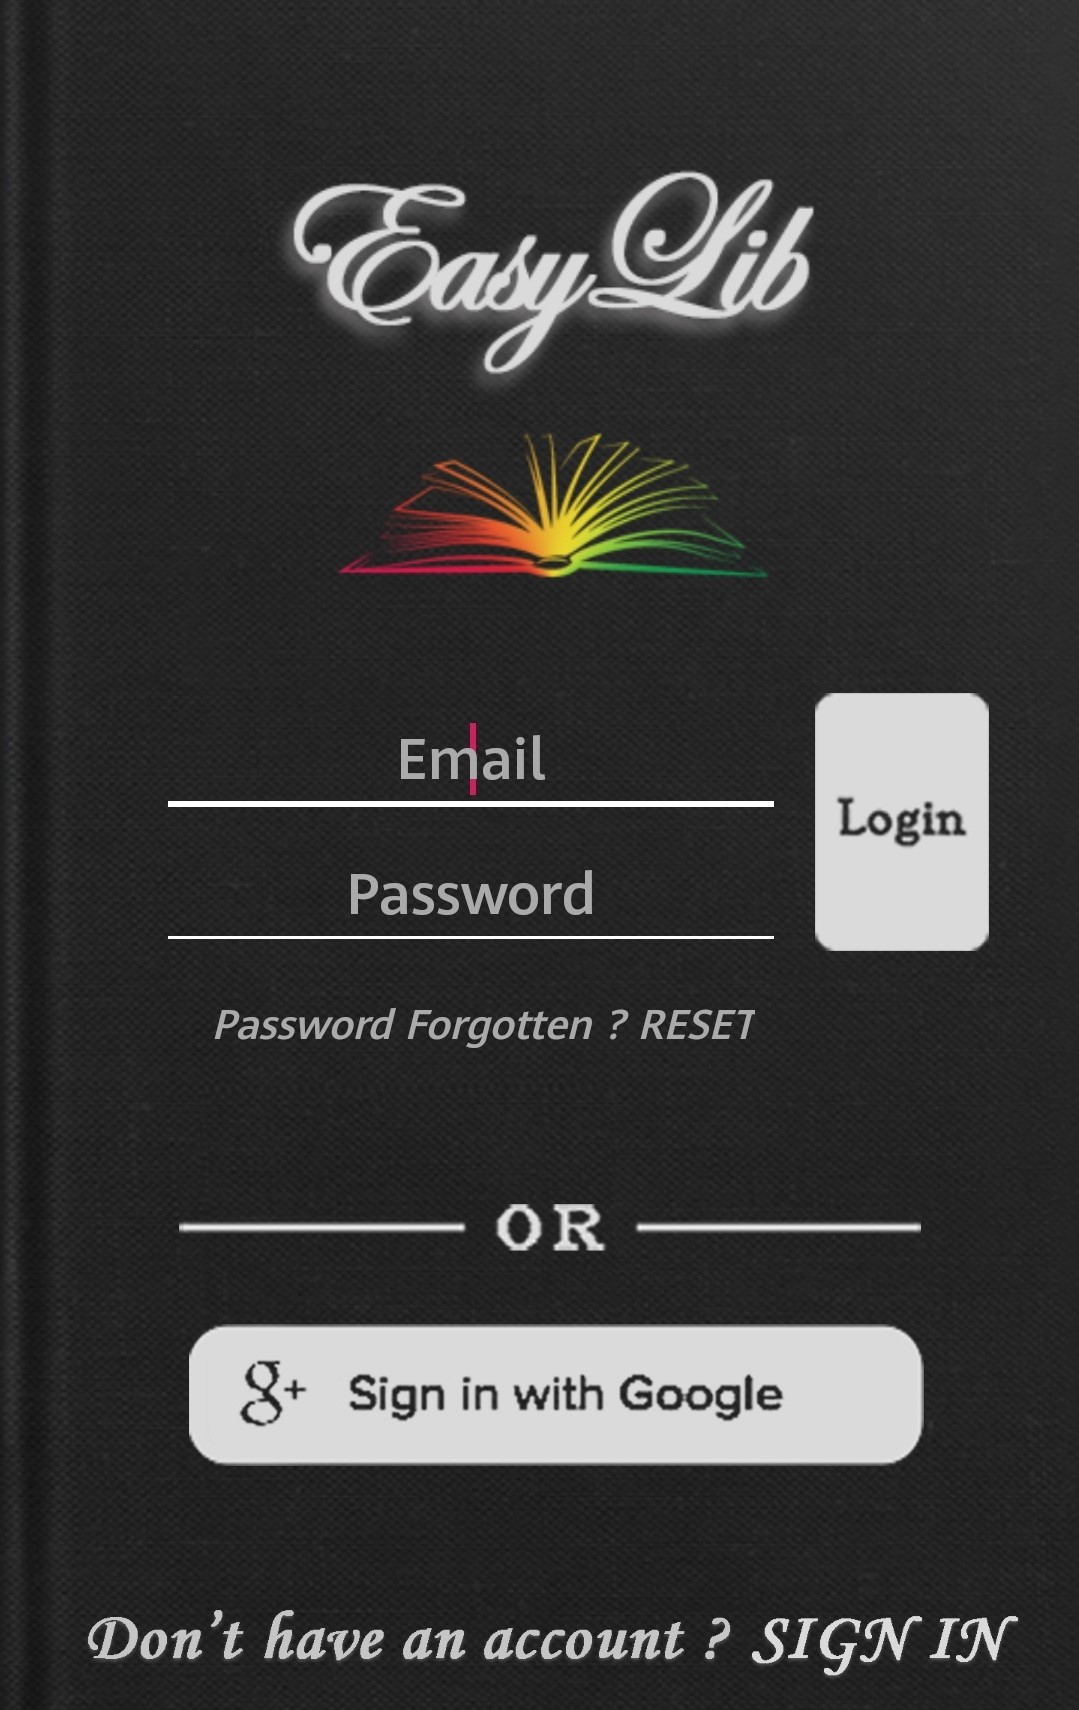
\includegraphics[scale=0.15]{Images/UI/Login_Register/1}
	\hspace{0.5cm}
	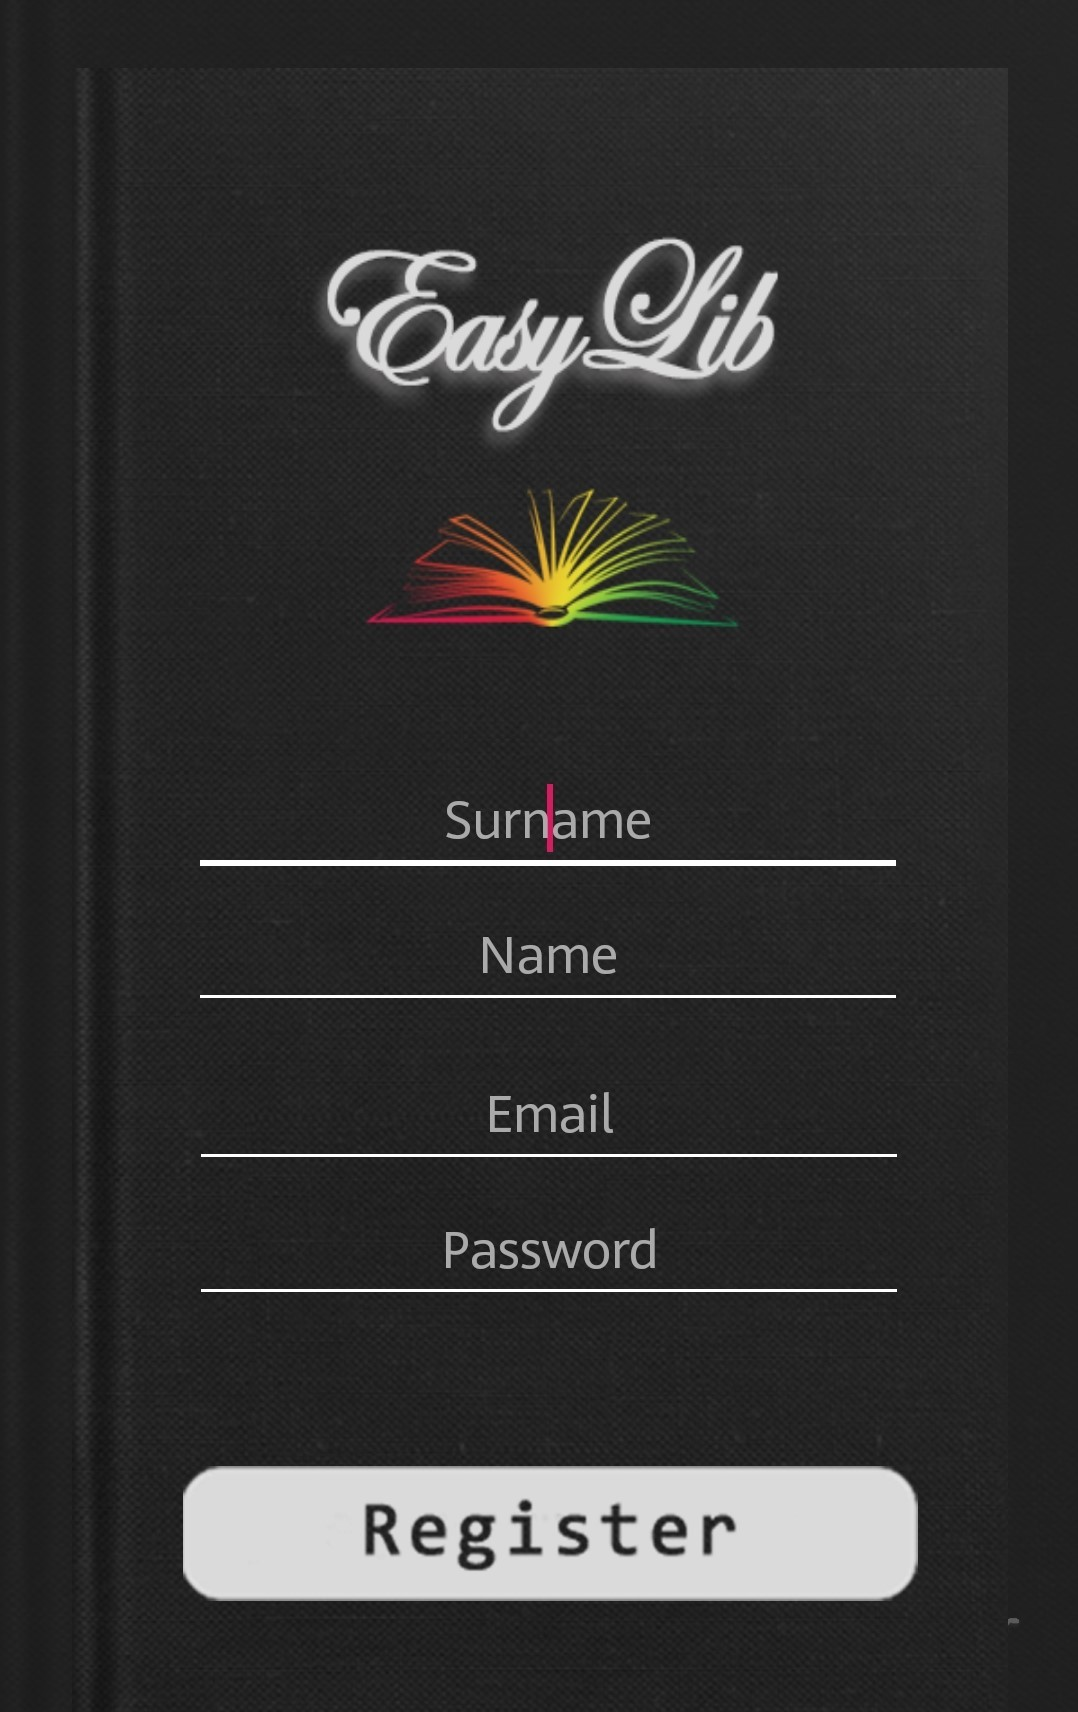
\includegraphics[scale=0.15]{Images/UI/Login_Register/2}
	\hspace{0.5cm}
	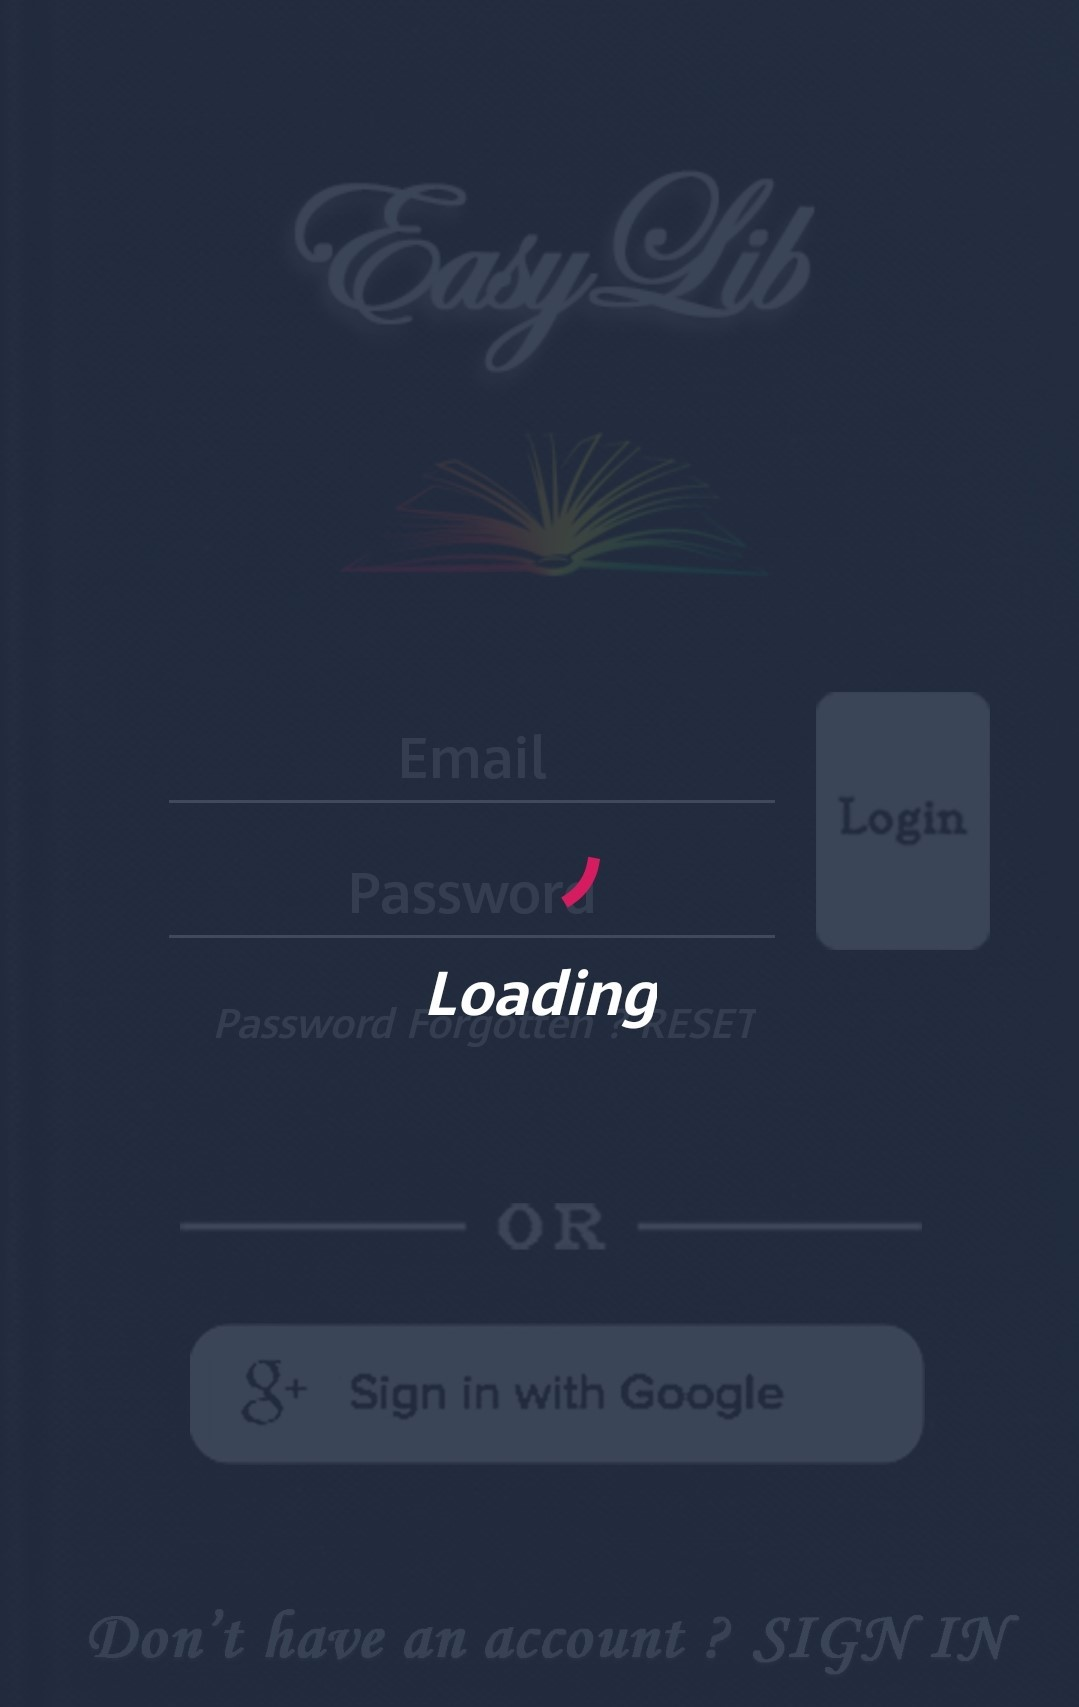
\includegraphics[scale=0.15]{Images/UI/Login_Register/3}
	\caption{Login \& Registration - UI}
\end{figure}

\vspace{3mm}
\mysubsubsection{Libraries + Set Favourite}
On MainActivity with the Home Fragment (Image 1) the user can see the Libraries that he has set as favourite and open them in order to see their content. Otherwise he can tap on "All Libraries" button and the list of the all available ones will appear (Image 2).\par
Once a library is selected the LibraryActivity will open up showing at the top the library information and its contents underneath (news, events, books). At the end a button will be shown in order to make the user able to set the library as Favourite / remove it from Favourites (Image 3).
\begin{figure}[H]
	\centering
	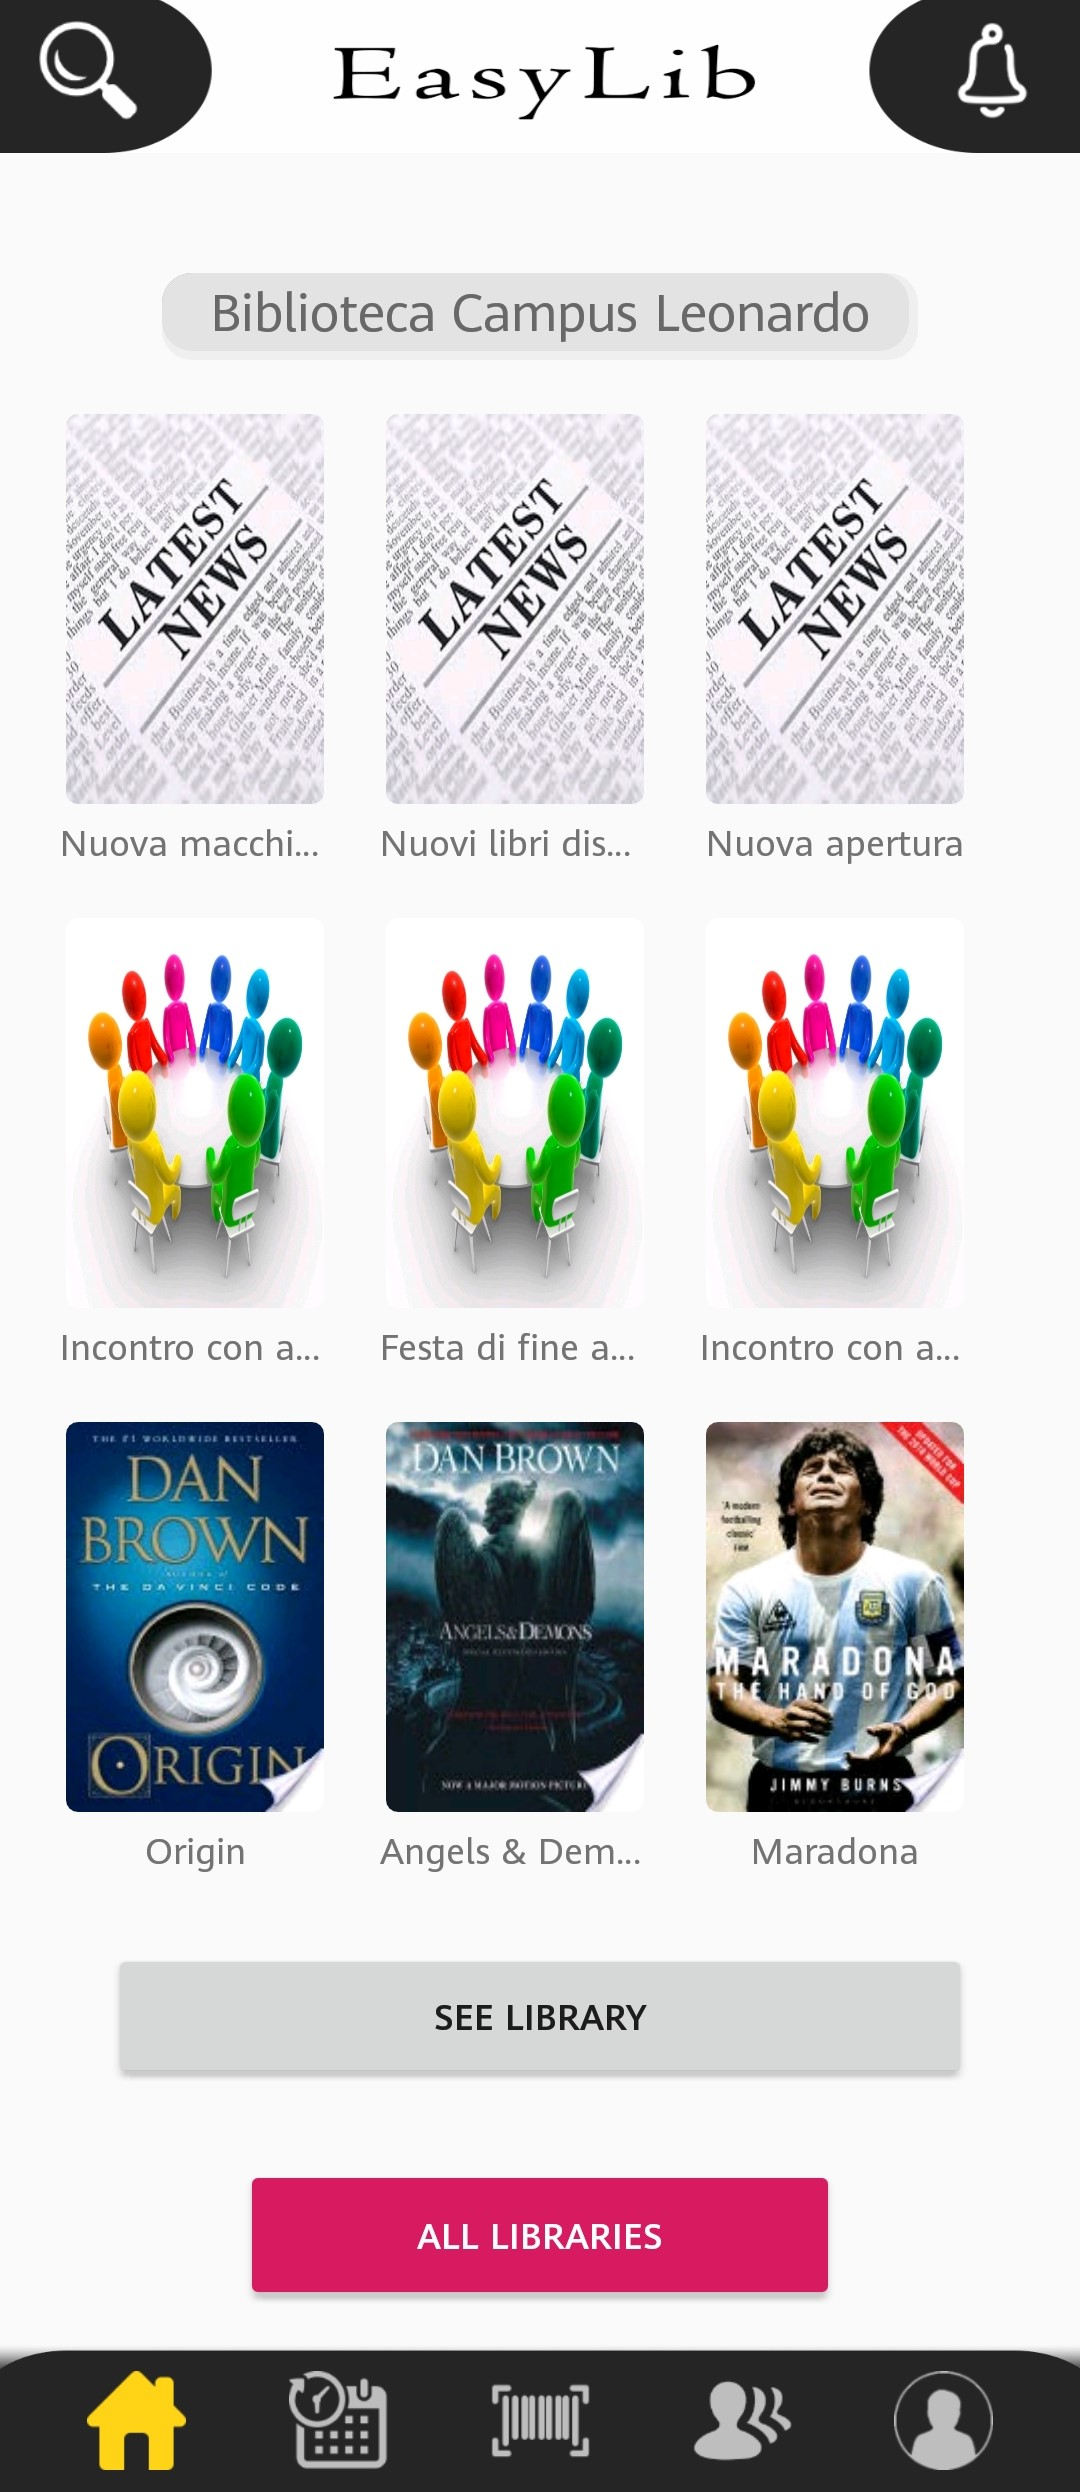
\includegraphics[scale=0.15]{Images/UI/Libraries/1}
	\hspace{0.5cm}
	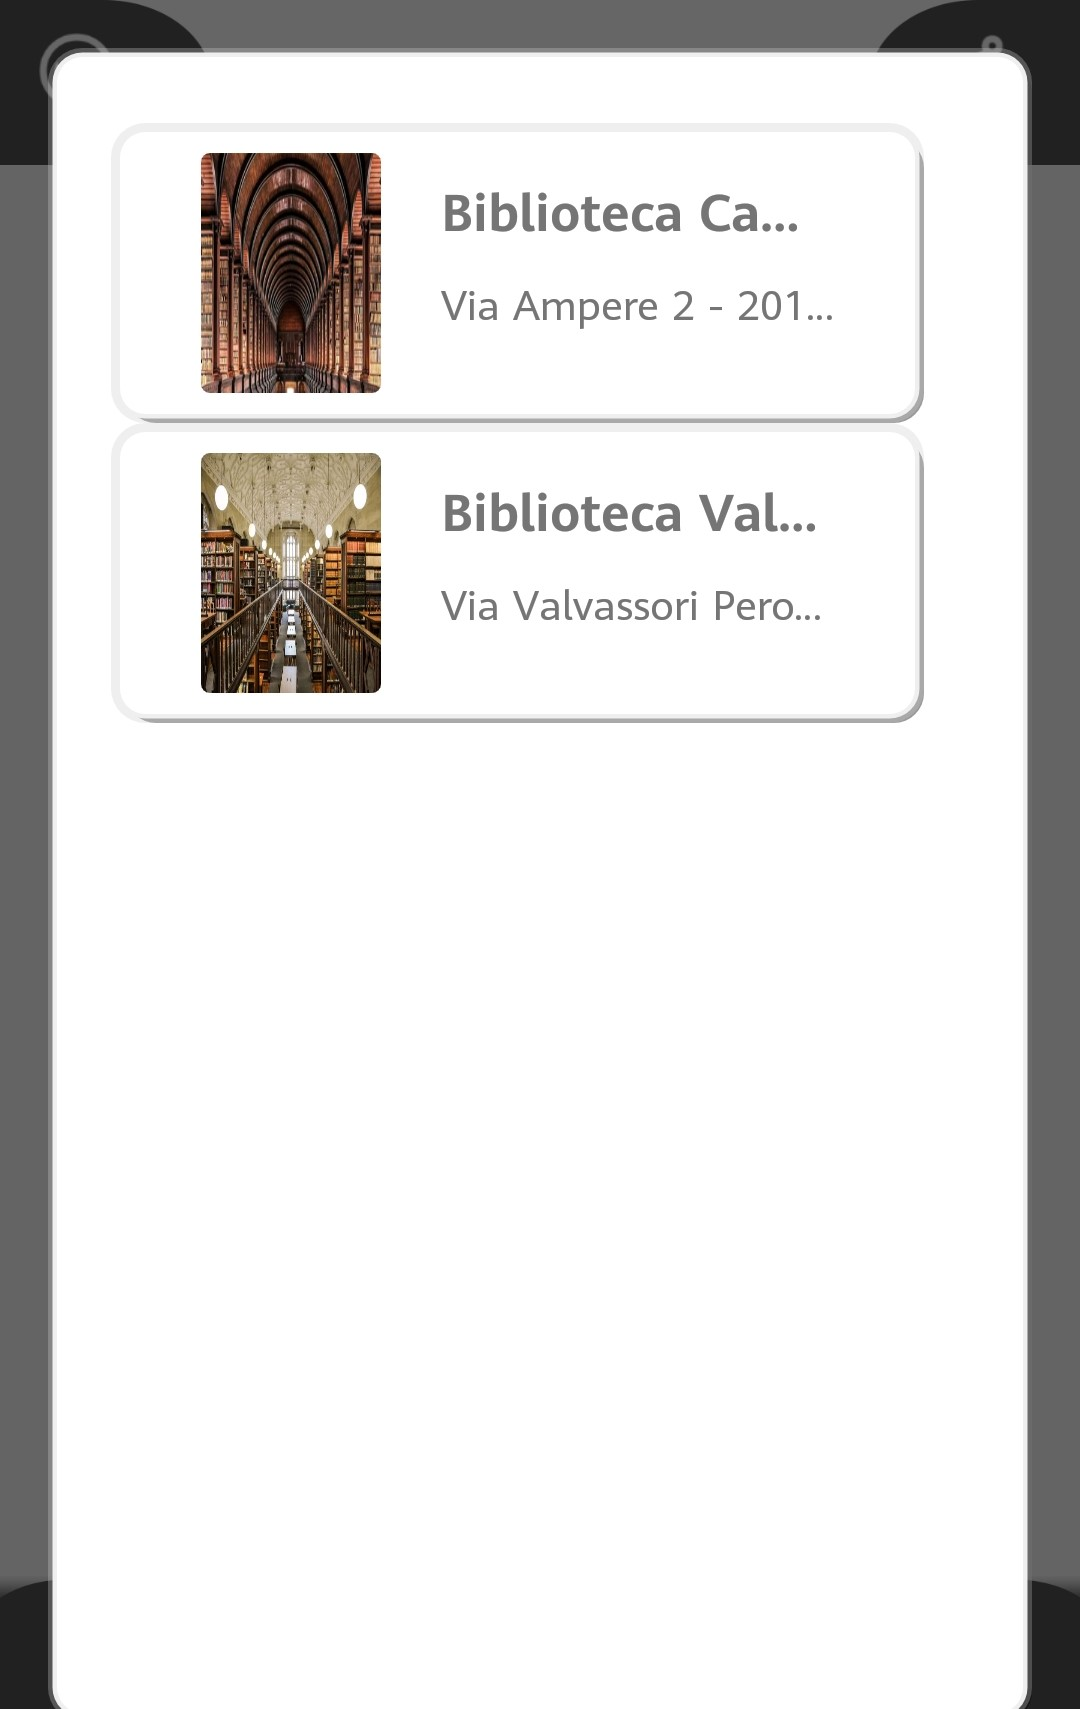
\includegraphics[scale=0.15]{Images/UI/Libraries/2}
	\hspace{0.5cm}
	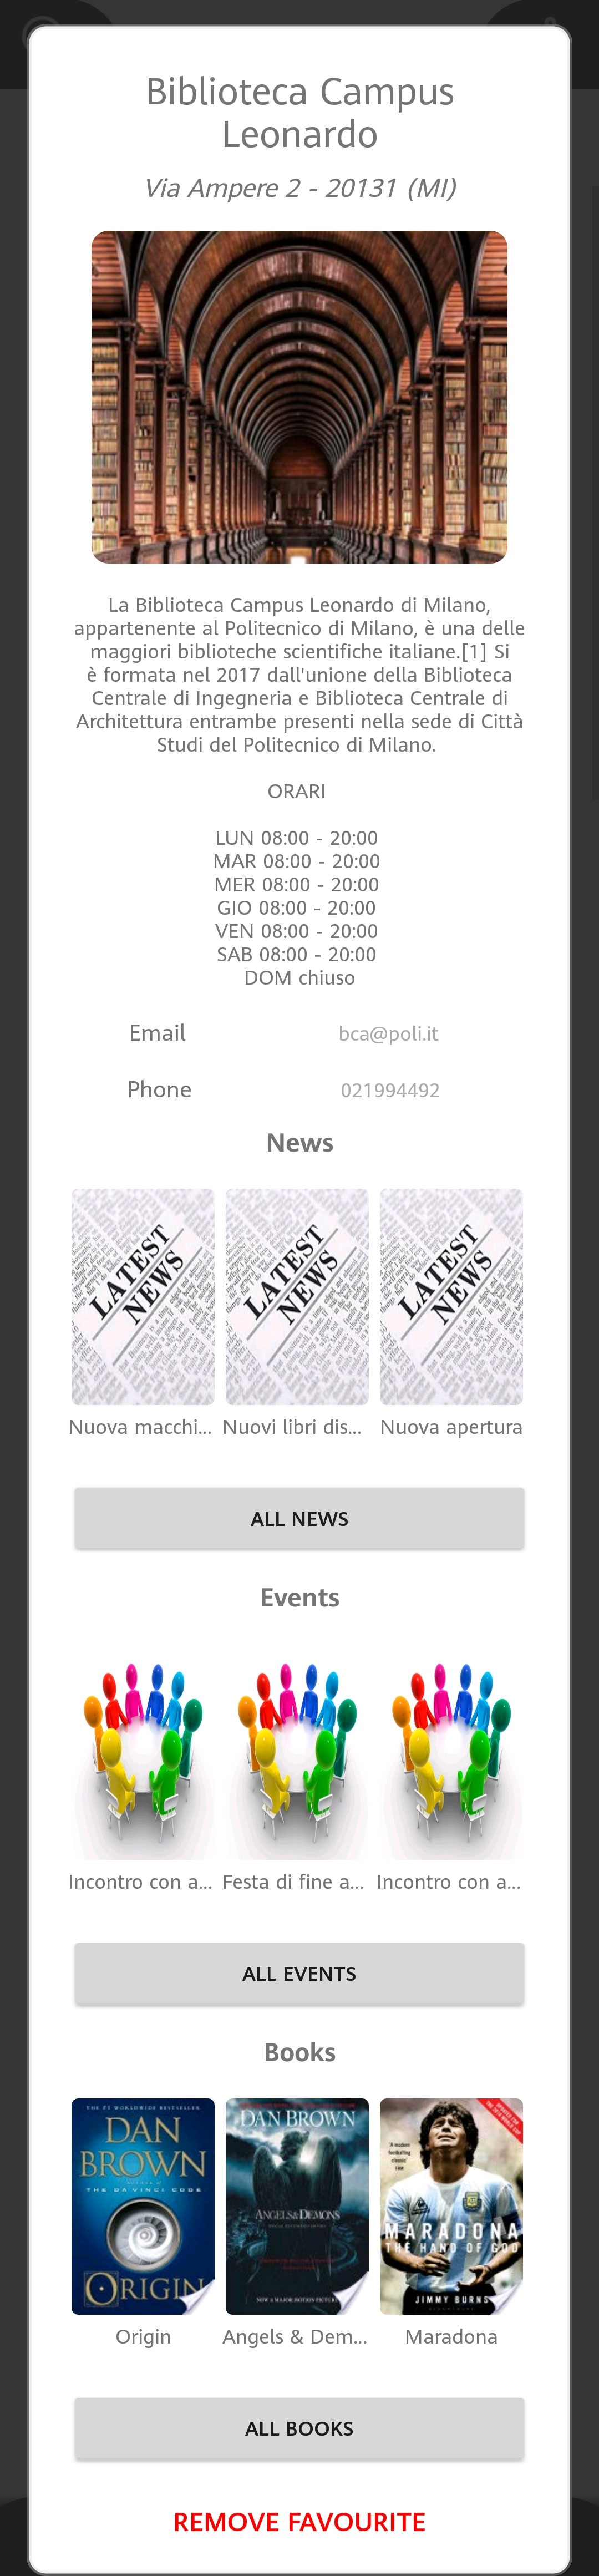
\includegraphics[scale=0.15]{Images/UI/Libraries/3}
	\caption{Libraries + Set Favourite - UI}
\end{figure}

\newpage
\mysubsubsection{Events + Reserve Seat}
As previously seen, inside the LibraryActivity the events organized by the library are shown. The user can open them and see their info (Image 1). Moreover in case there are still available seats he can reserve one of them.\par
All the events joined by the user are shown on the Profile (Image 2).
\begin{figure}[H]
	\centering
	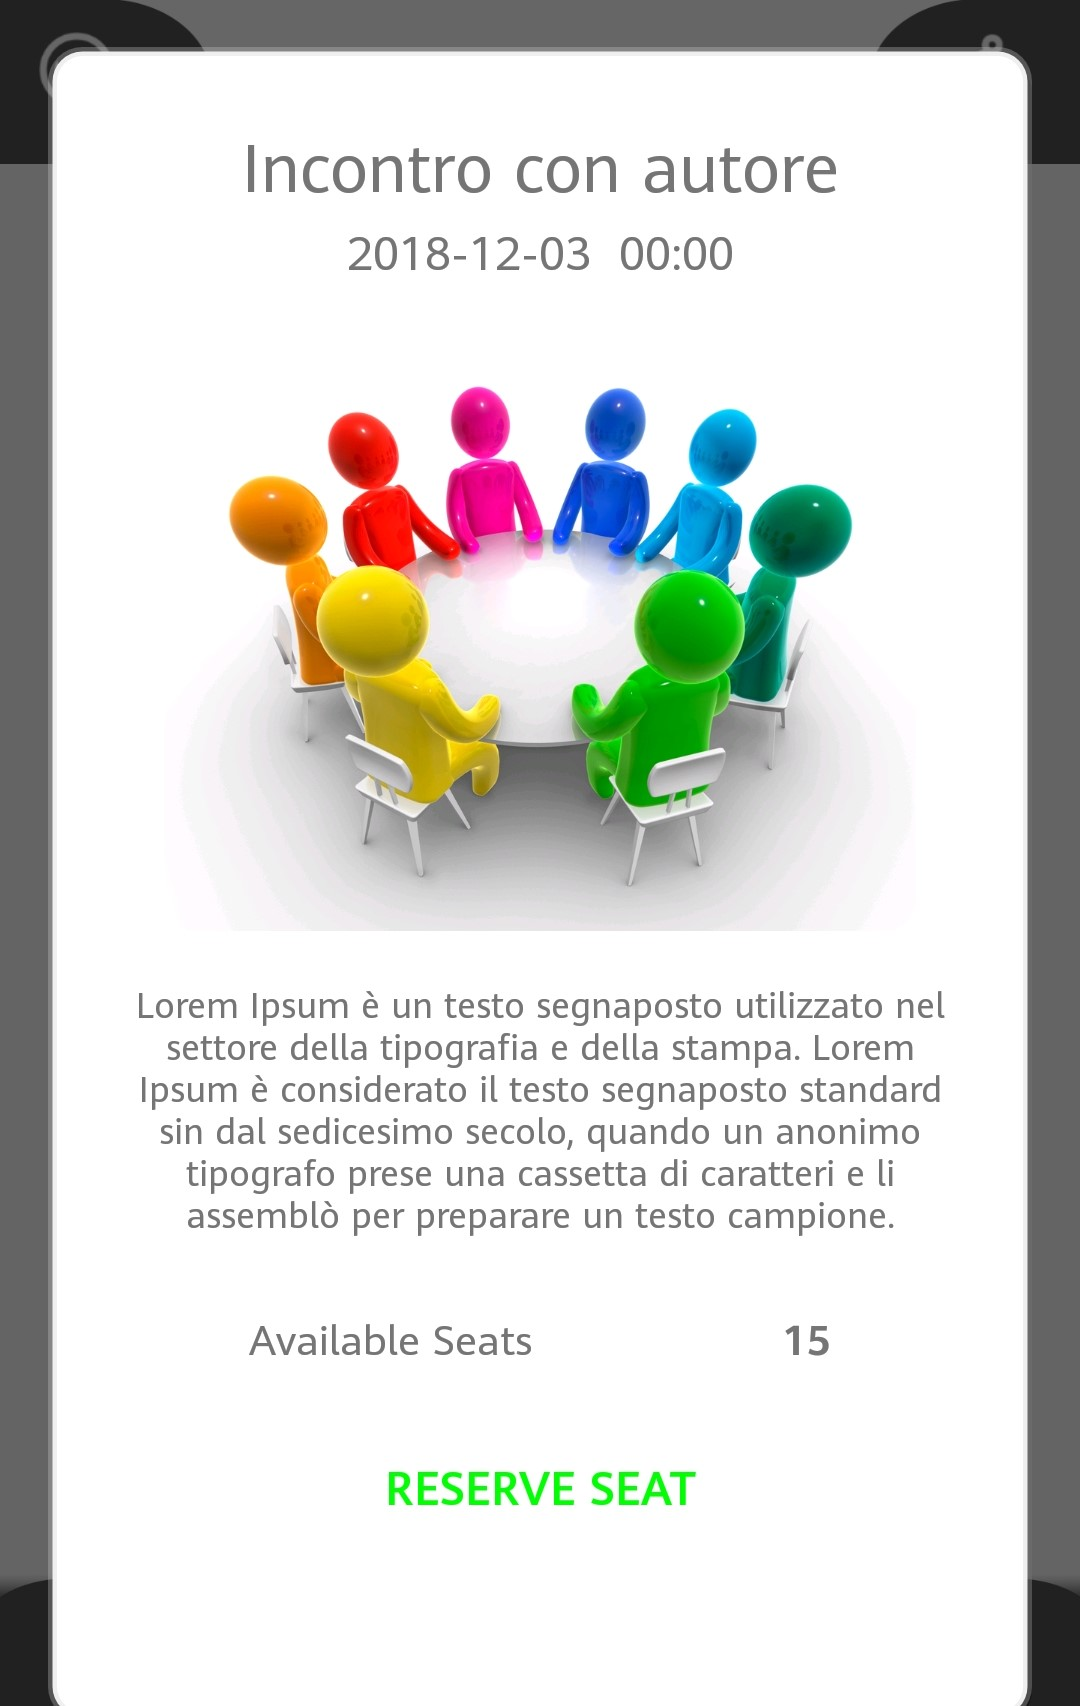
\includegraphics[scale=0.15]{Images/UI/Events/1}
	\hspace{0.5cm}
	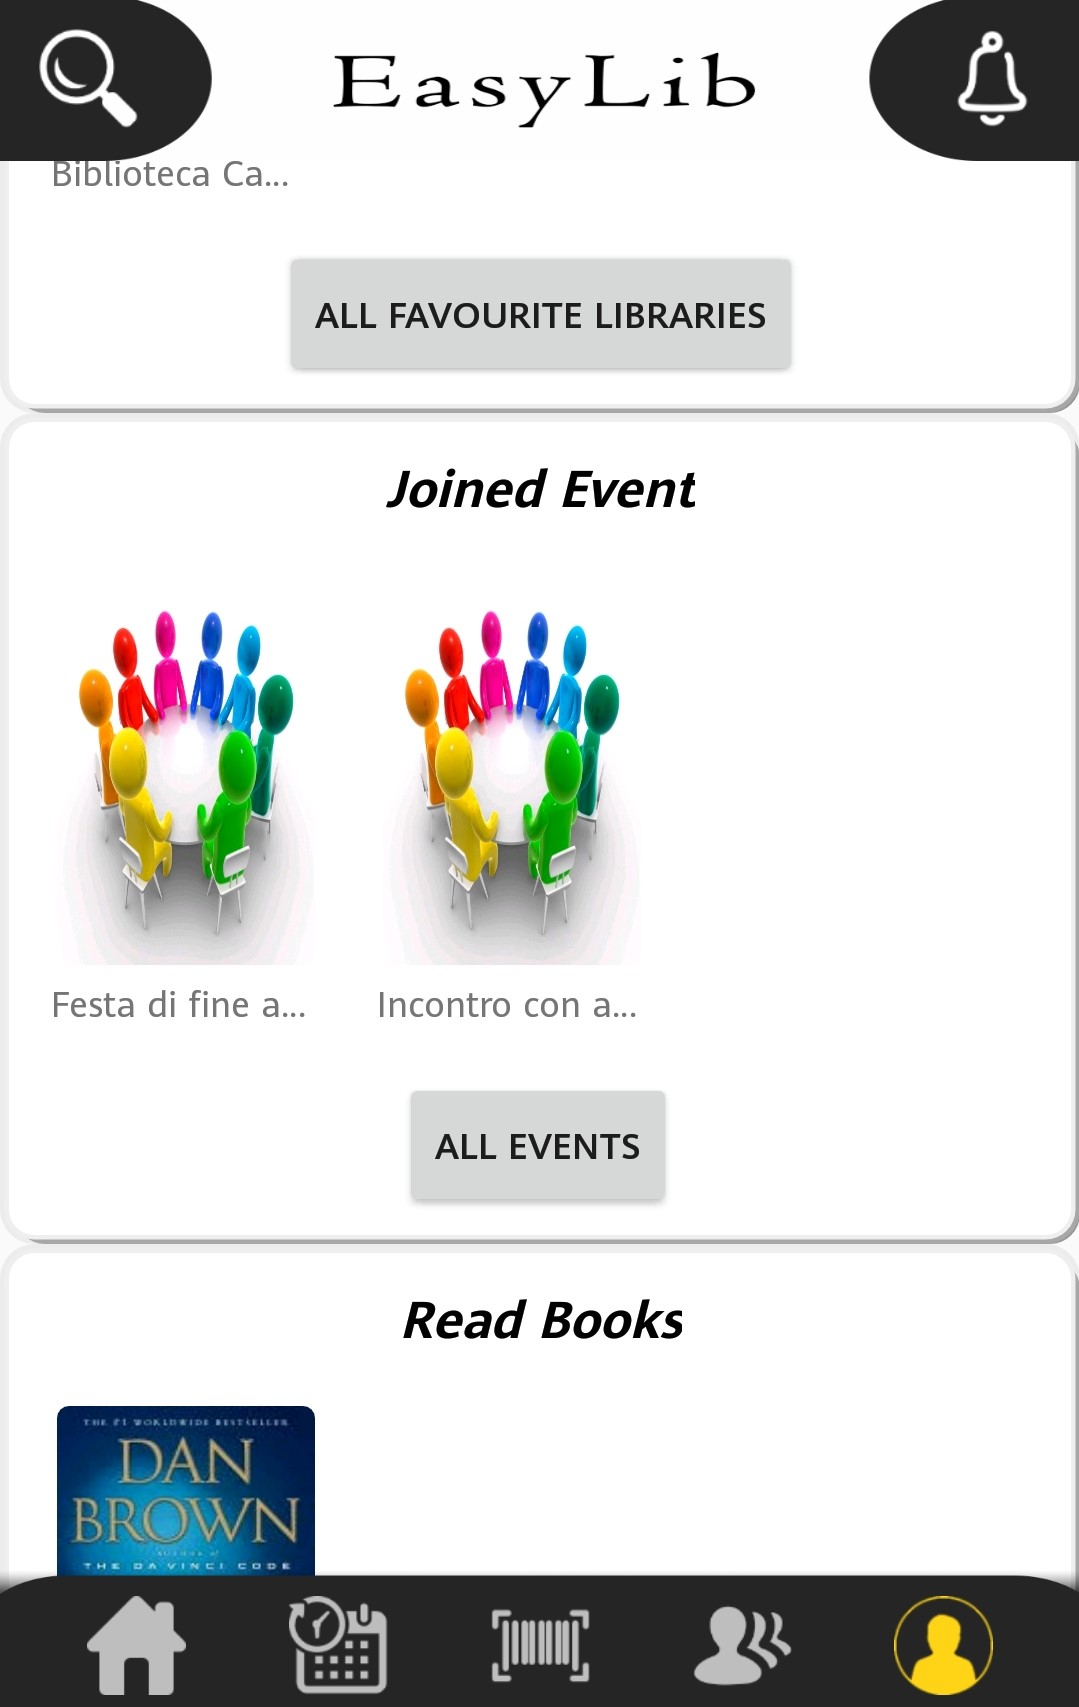
\includegraphics[scale=0.15]{Images/UI/Events/2}
	\caption{Events + Reserve Seat - UI}
\end{figure}

\newpage
\mysubsubsection{Search Books}
There are 2 ways to search for a book :
\begin{itemize}
	\item \emph{By Title/Author/Genre :} the user can tap the "Search Icon" on top of the MainActivity (shown on the previous figures) and fill the Title field or activate the Advanced Search fields (Image 1).
	\item \emph{QR code :} in the bottom NavBar on MainActivity there is a "Scan Icon" that when tapped opens up an activity that activates the camera and scans the qr-code (Image 2).
\end{itemize}
\begin{figure}[H]
	\centering
	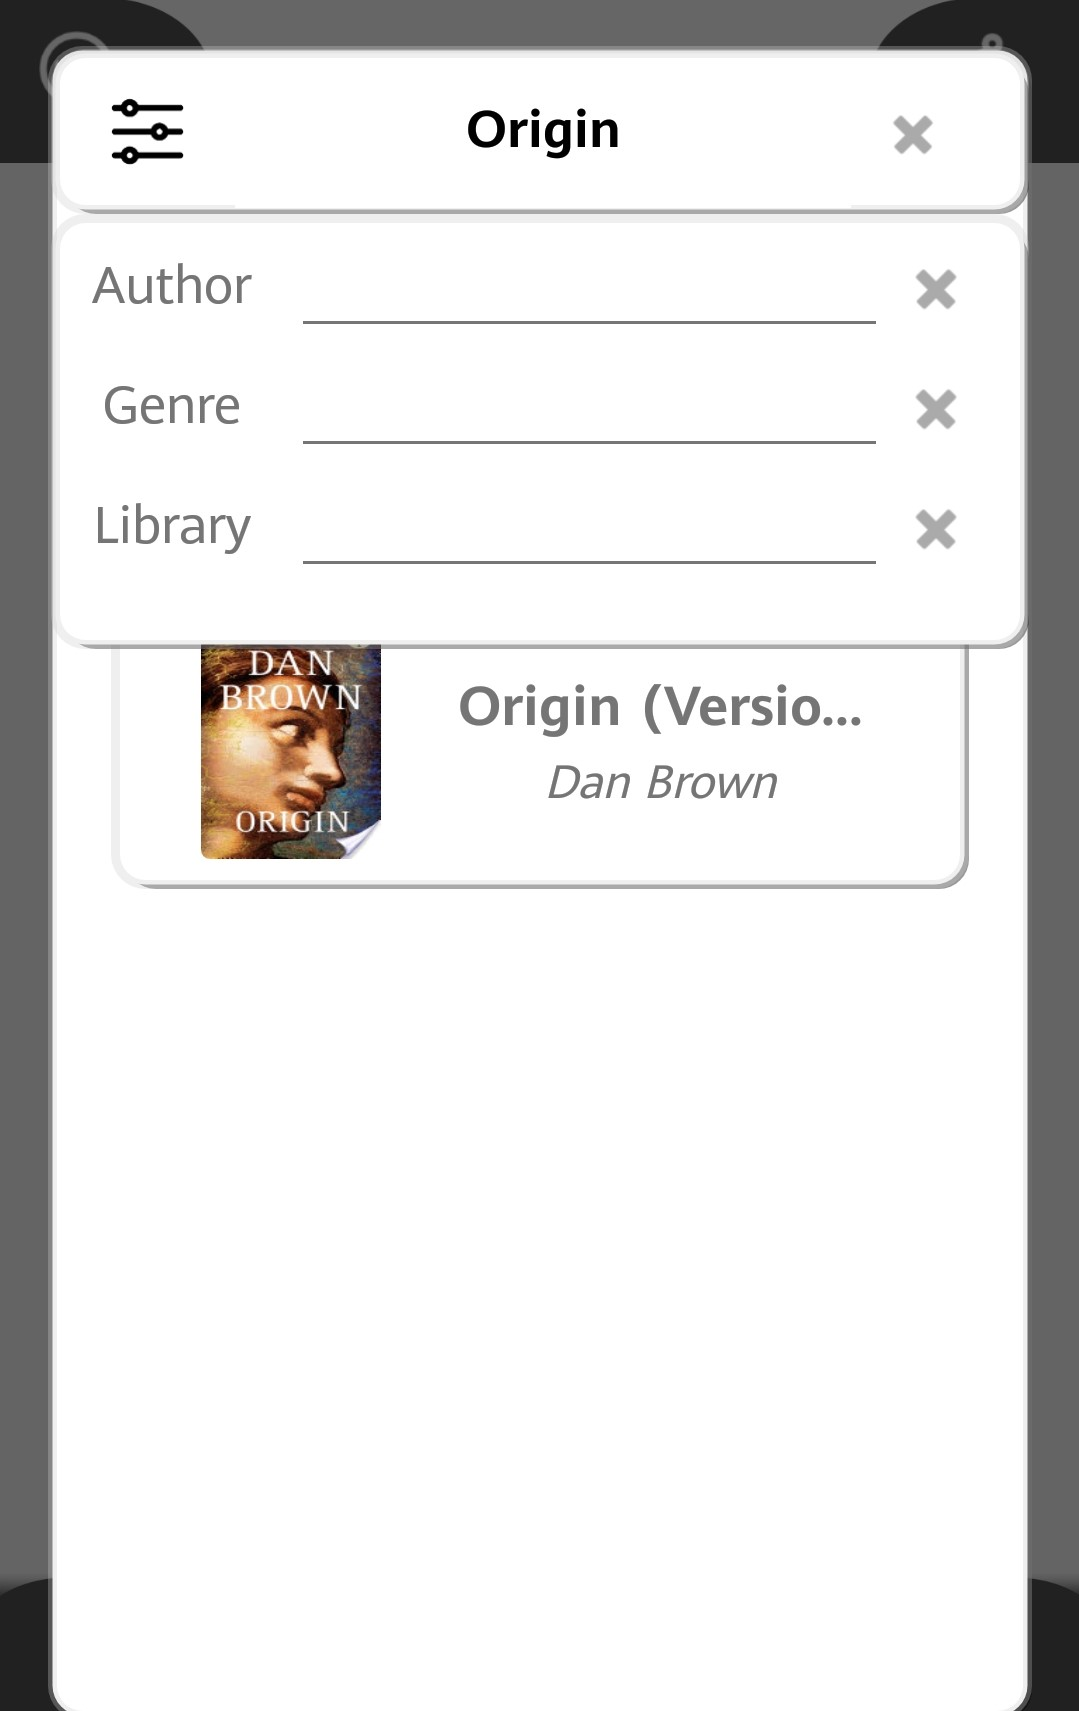
\includegraphics[scale=0.15]{Images/UI/Search/1}
	\hspace{0.5cm}
	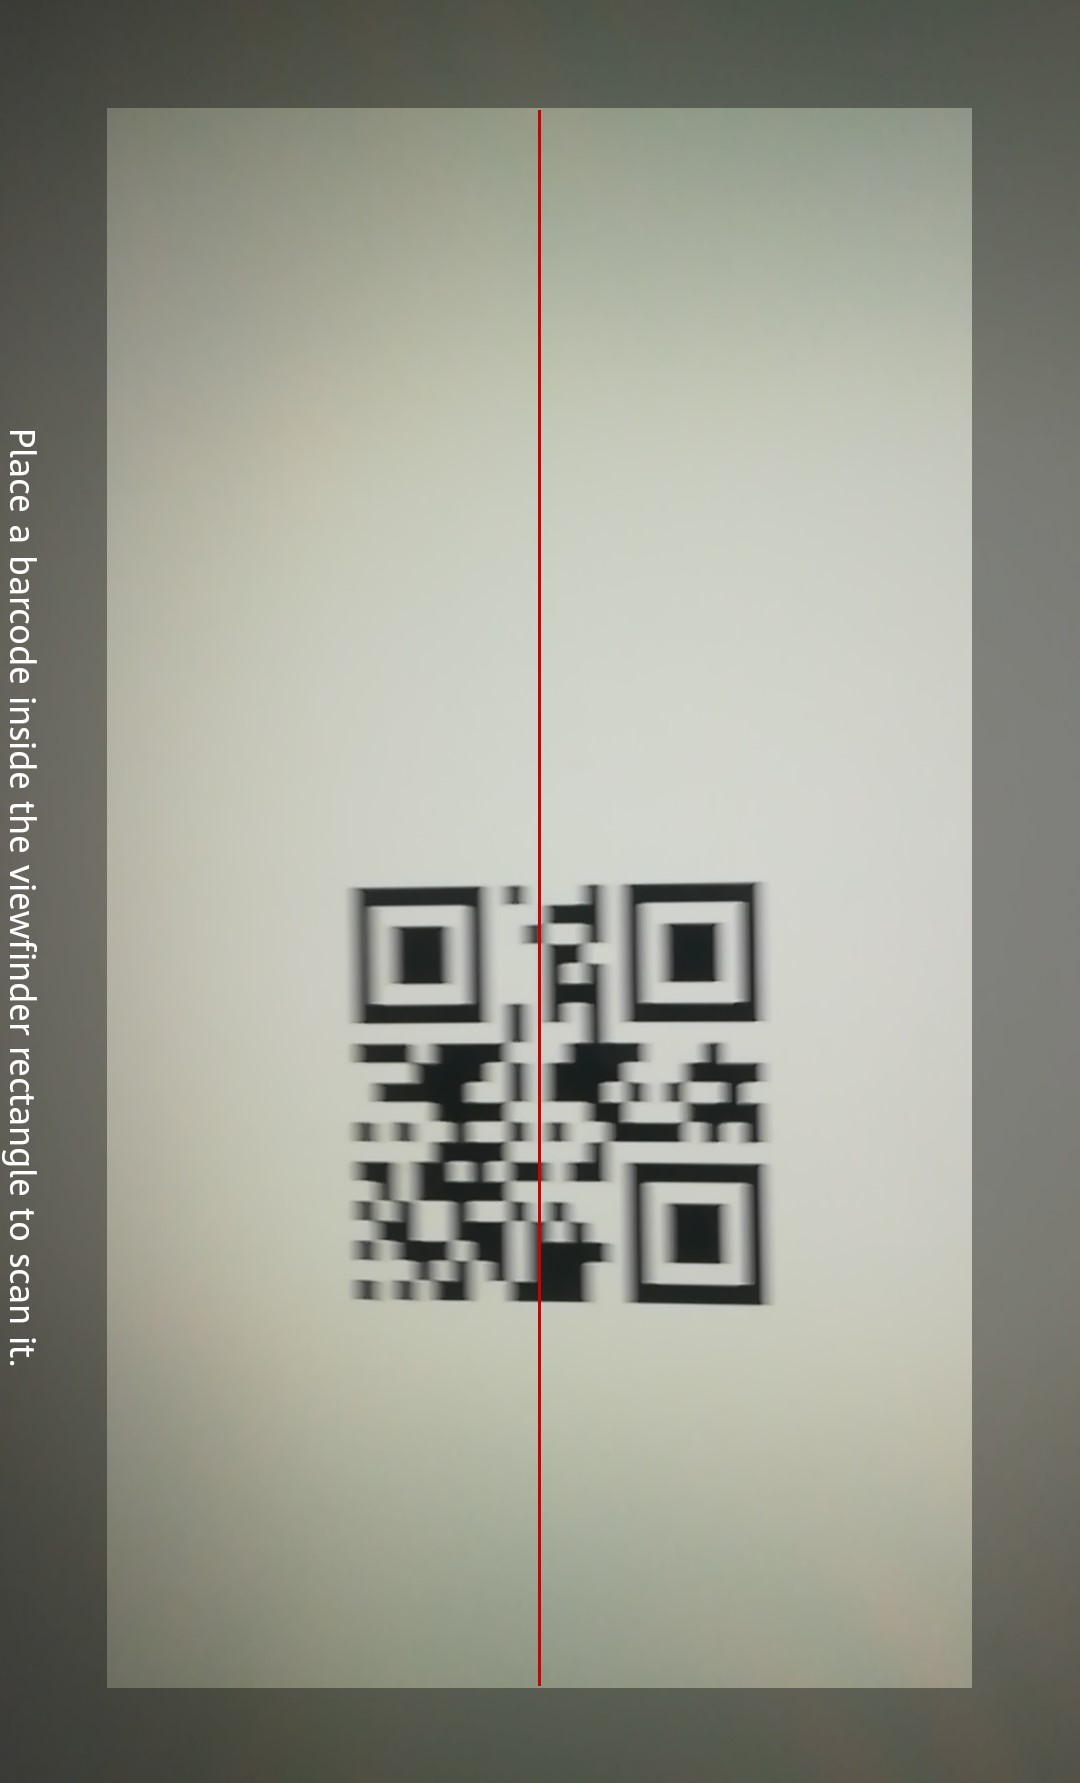
\includegraphics[scale=0.15]{Images/UI/Search/2}
	\caption{Search Books - UI}
\end{figure}

\newpage
\mysubsubsection{Books + Reservation}
Once the user selects a book the "BookActivity" opens up and shows him all book's information and image (Image 1). At the end it's displayed the current status of the book (if it's been already read or not) and the list of all the libraries where it's available (Image 2).\par
If the user wants, he can reserve the book by tapping the "Reserve" button and so the status is updated (Image 3).
\begin{figure}[H]
	\centering
	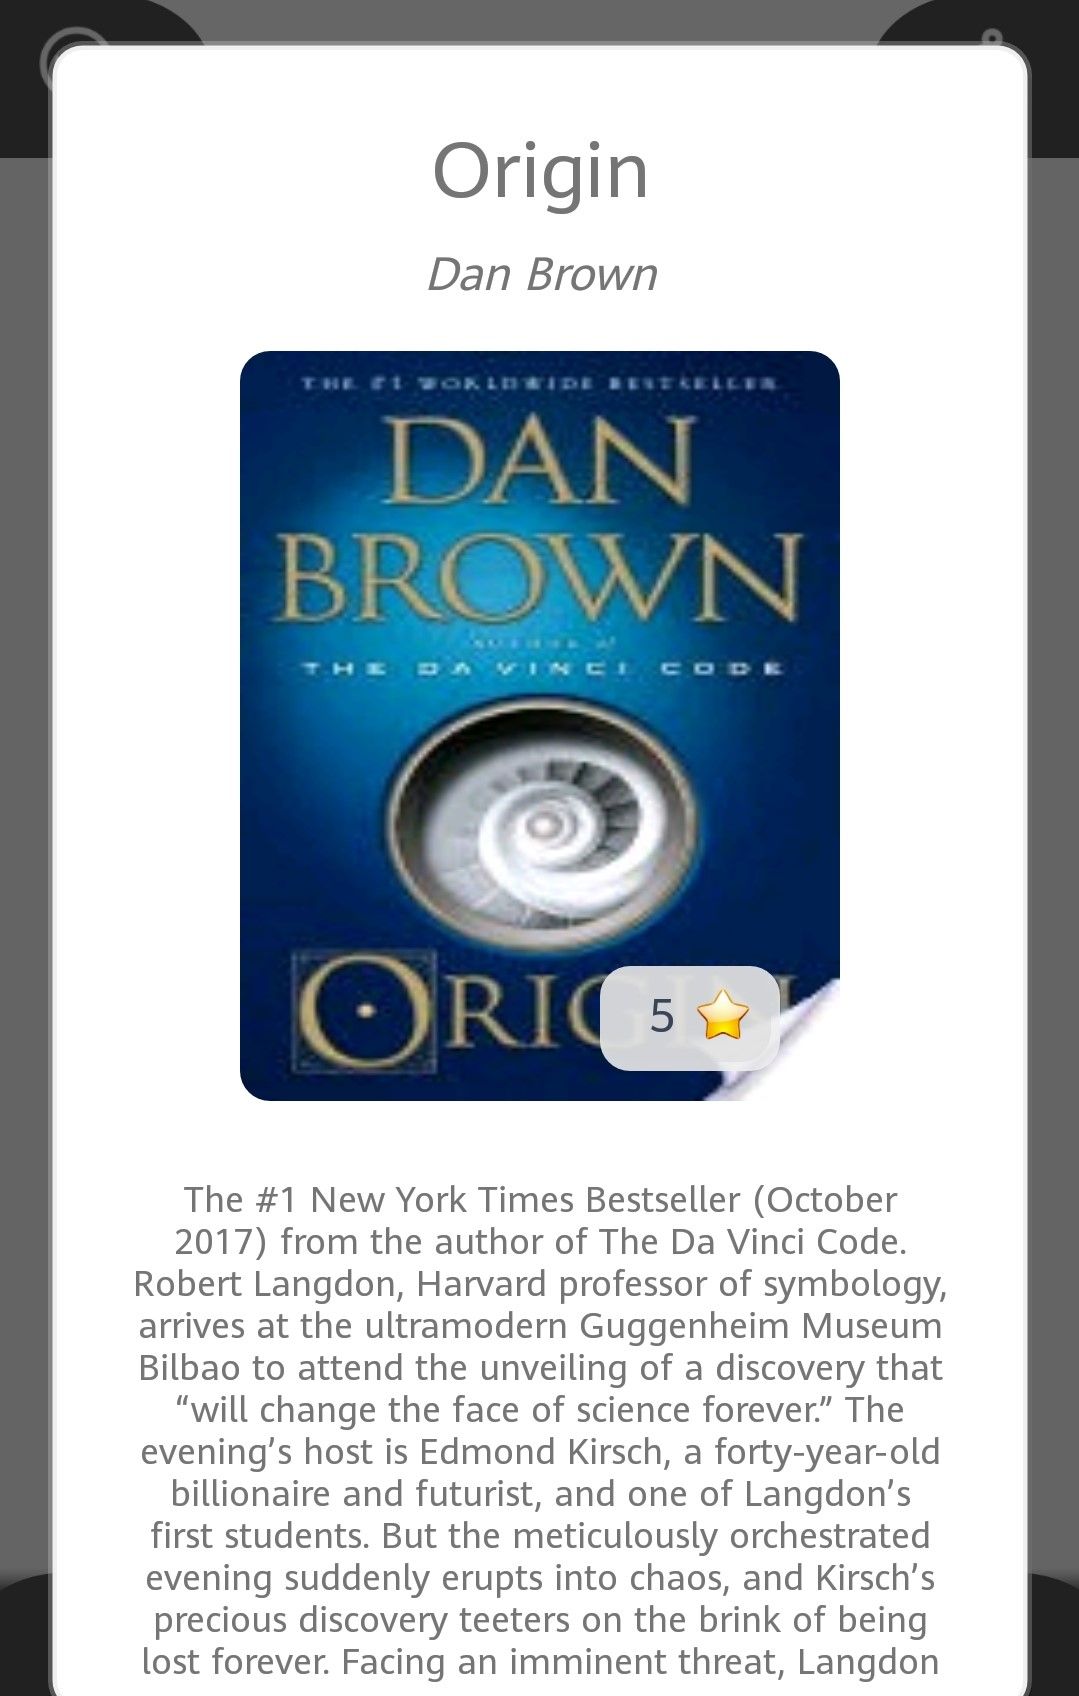
\includegraphics[scale=0.15]{Images/UI/Book/1}
	\hspace{0.5cm}
	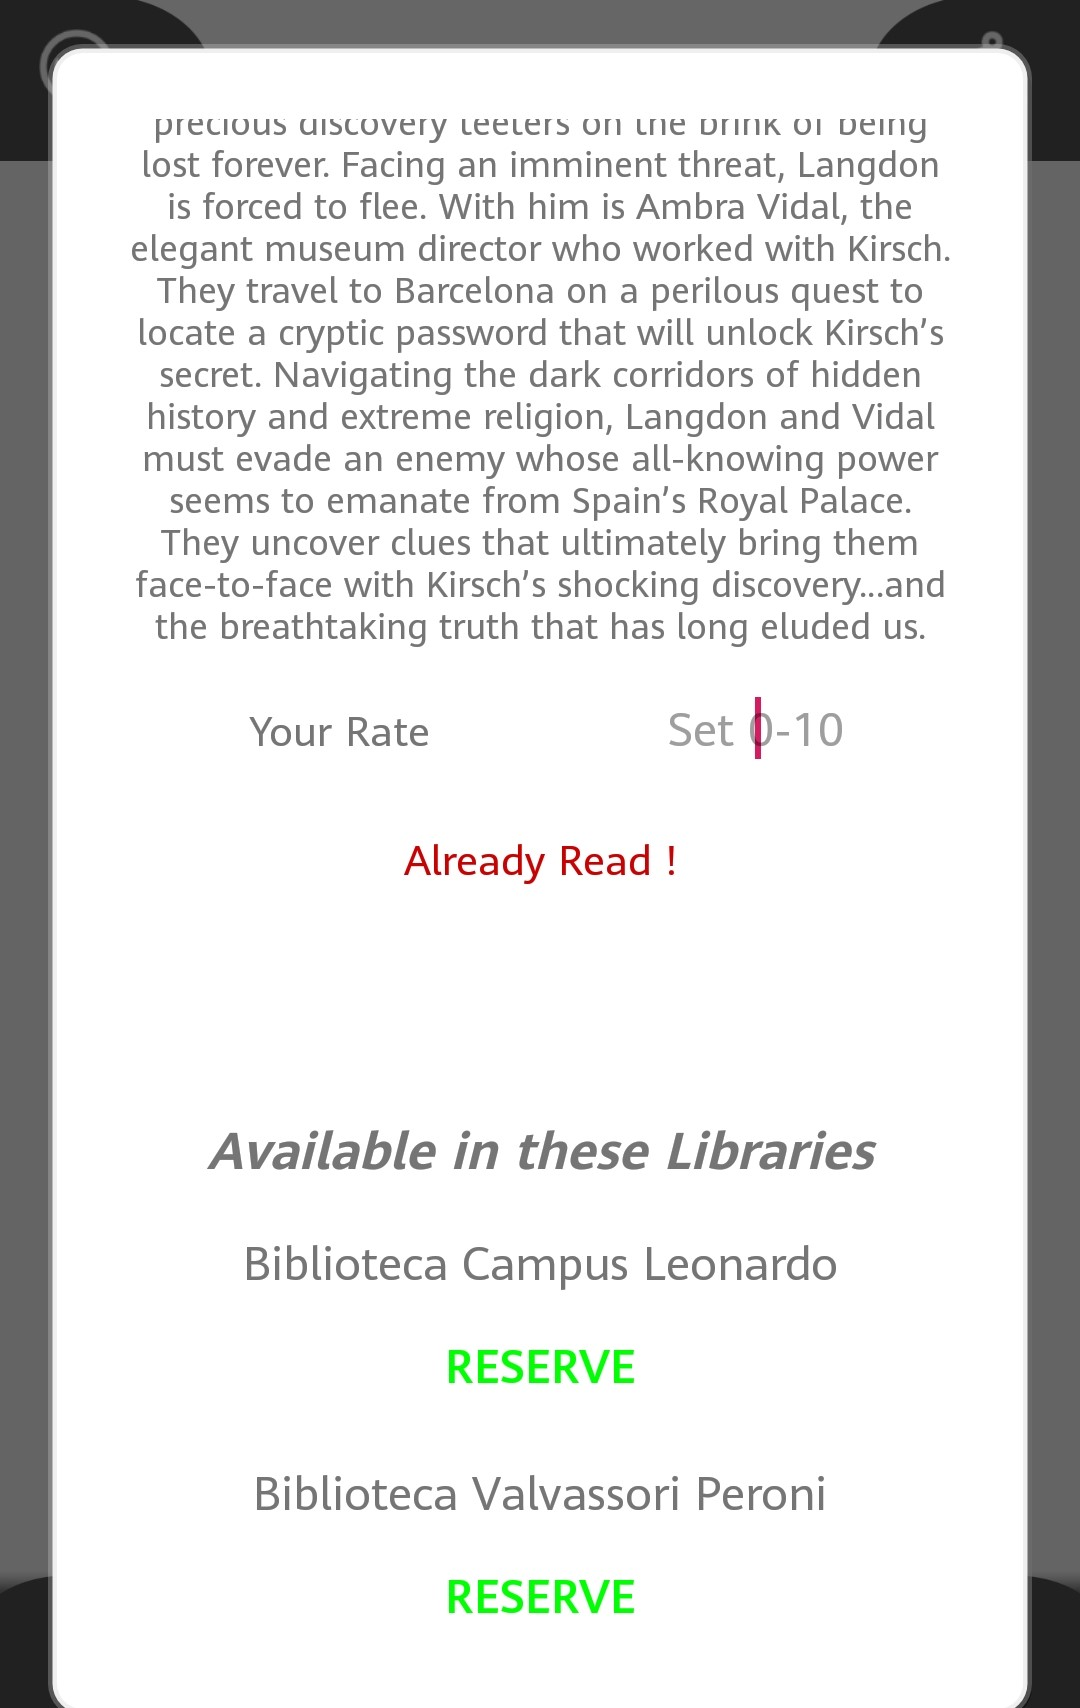
\includegraphics[scale=0.15]{Images/UI/Book/2}
	\hspace{0.5cm}
	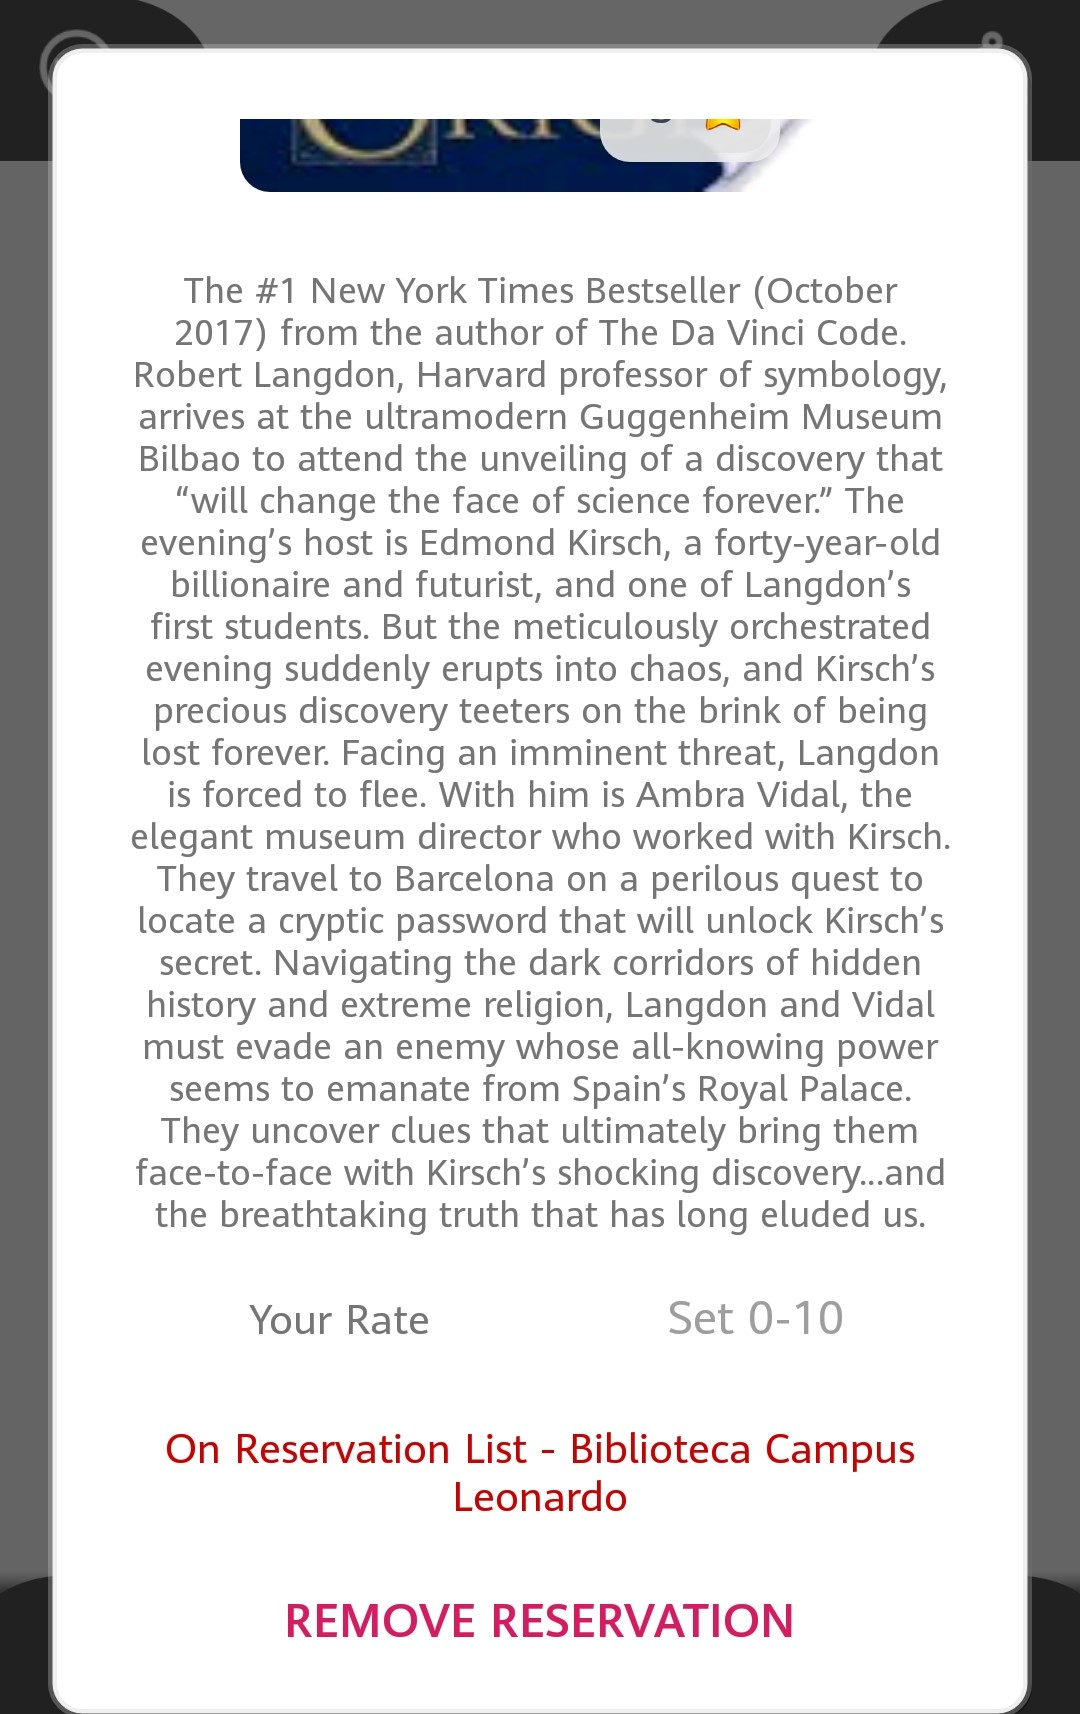
\includegraphics[scale=0.15]{Images/UI/Book/3}
	\caption{Books + Reservation - UI}
\end{figure}
\vspace*{0mm}
The user can do that only in case there are available books, in a specific library, and see all the reservations in the "Calendar Fragment" on "MainActivity" (Image 4). Otherwise the user is added on the Waiting List. All the books for which the user is on Waiting List are shown on the "Queue Fragment" on "MainActivity" with the relative position on queue (Image 5).
\begin{figure}[H]
	\centering
	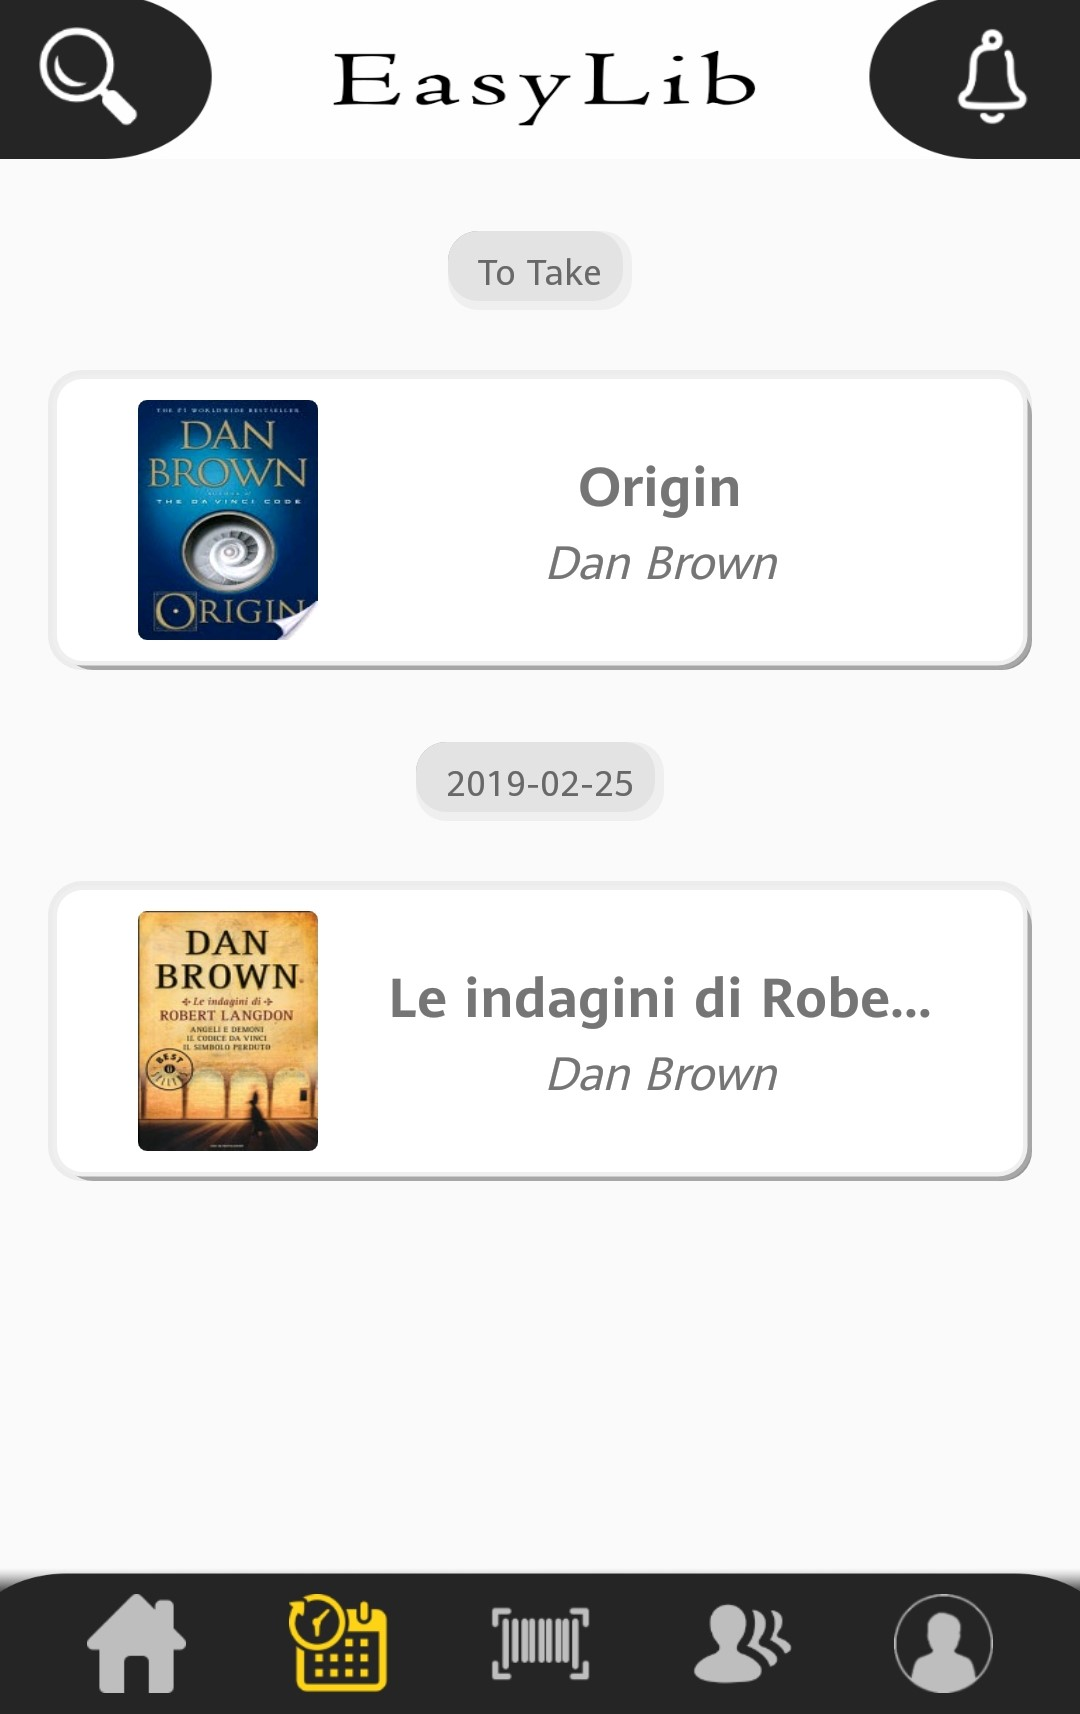
\includegraphics[scale=0.15]{Images/UI/Book/4}
	\hspace{0.5cm}
	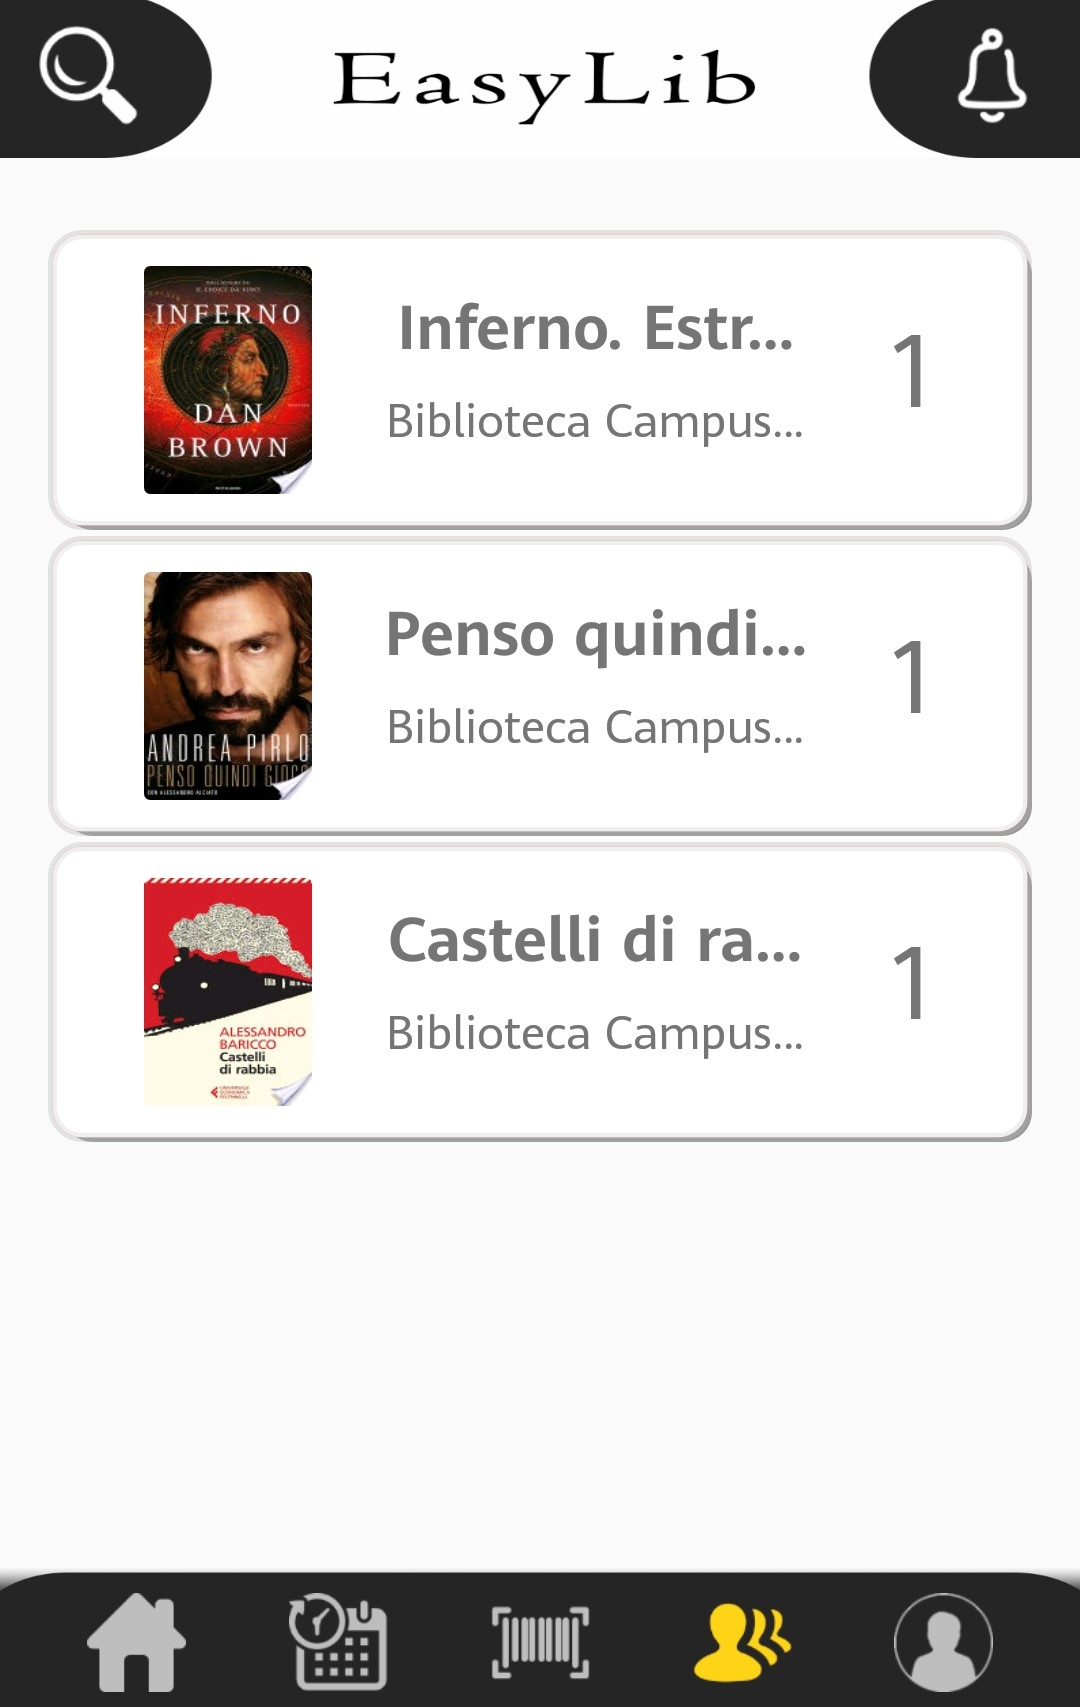
\includegraphics[scale=0.15]{Images/UI/Book/5}
	\caption{Calendar \& Queue - UI}
\end{figure}

\newpage
\mysubsubsection{Profile}
The user can see all his information on the "Profile Fragment" on "Main Activity", also his USER ID (Image 1).\par
He can also see : all his Favourite Libraries, all the Joined Events and all the Read Books (Image 2).\par
In case of necessity he can also modify it's credentials by tapping the "Edit Icon" on top of the "Profile Fragment" and by filling up the form shown on the "Edit Profile Activity" (Image 3).
\vspace*{1cm}
\begin{figure}[H]
	\centering
	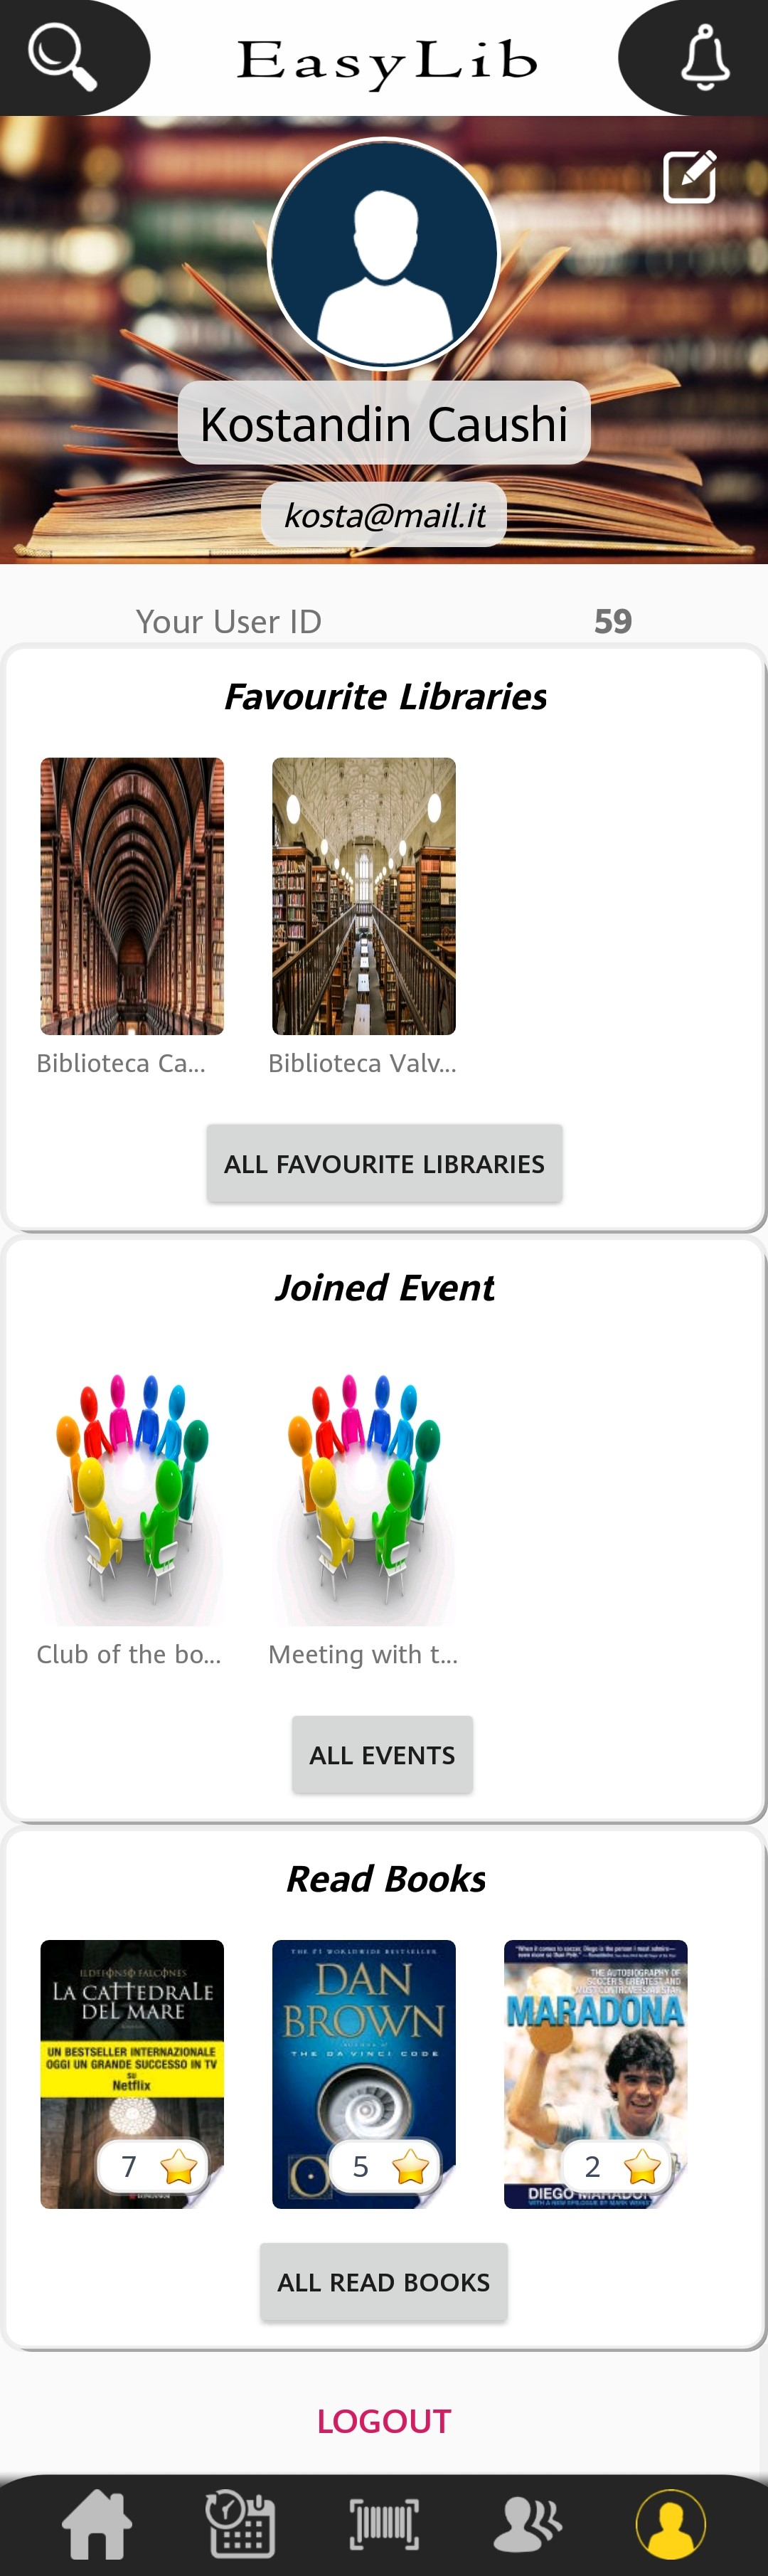
\includegraphics[scale=0.15]{Images/UI/Profile/1}
	\hspace{0.5cm}
	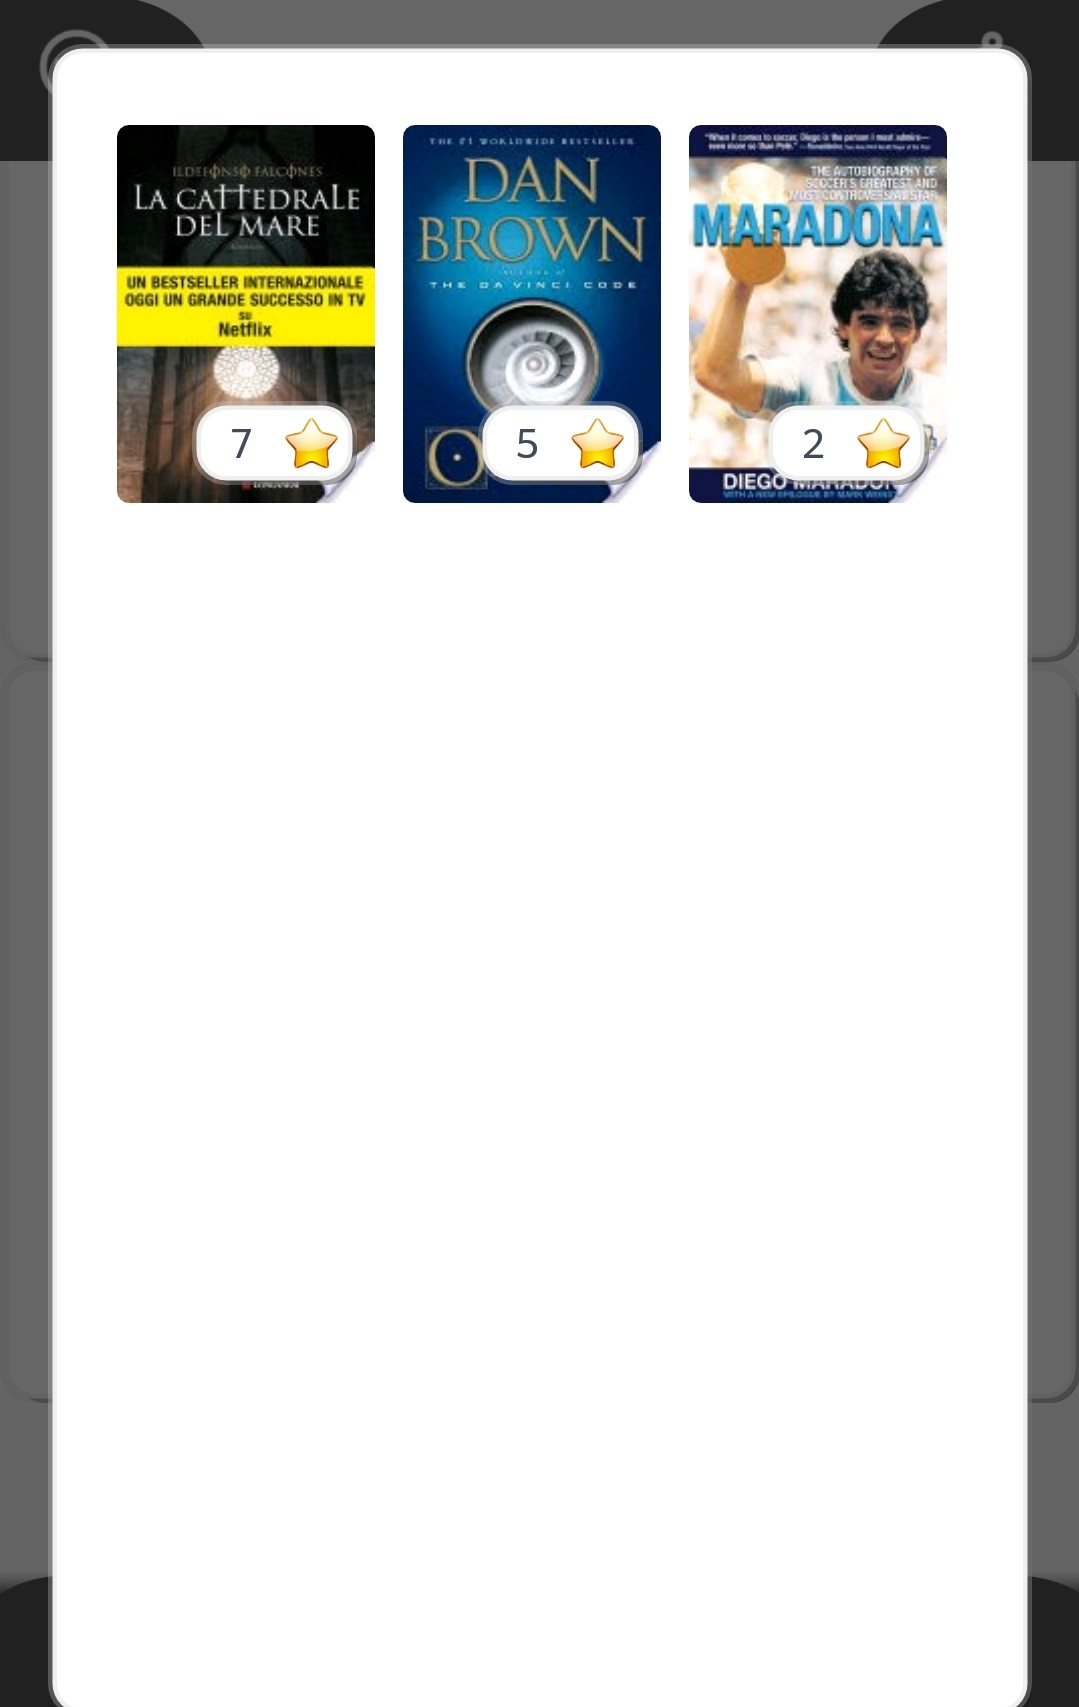
\includegraphics[scale=0.15]{Images/UI/Profile/2}
	\hspace{0.5cm}
	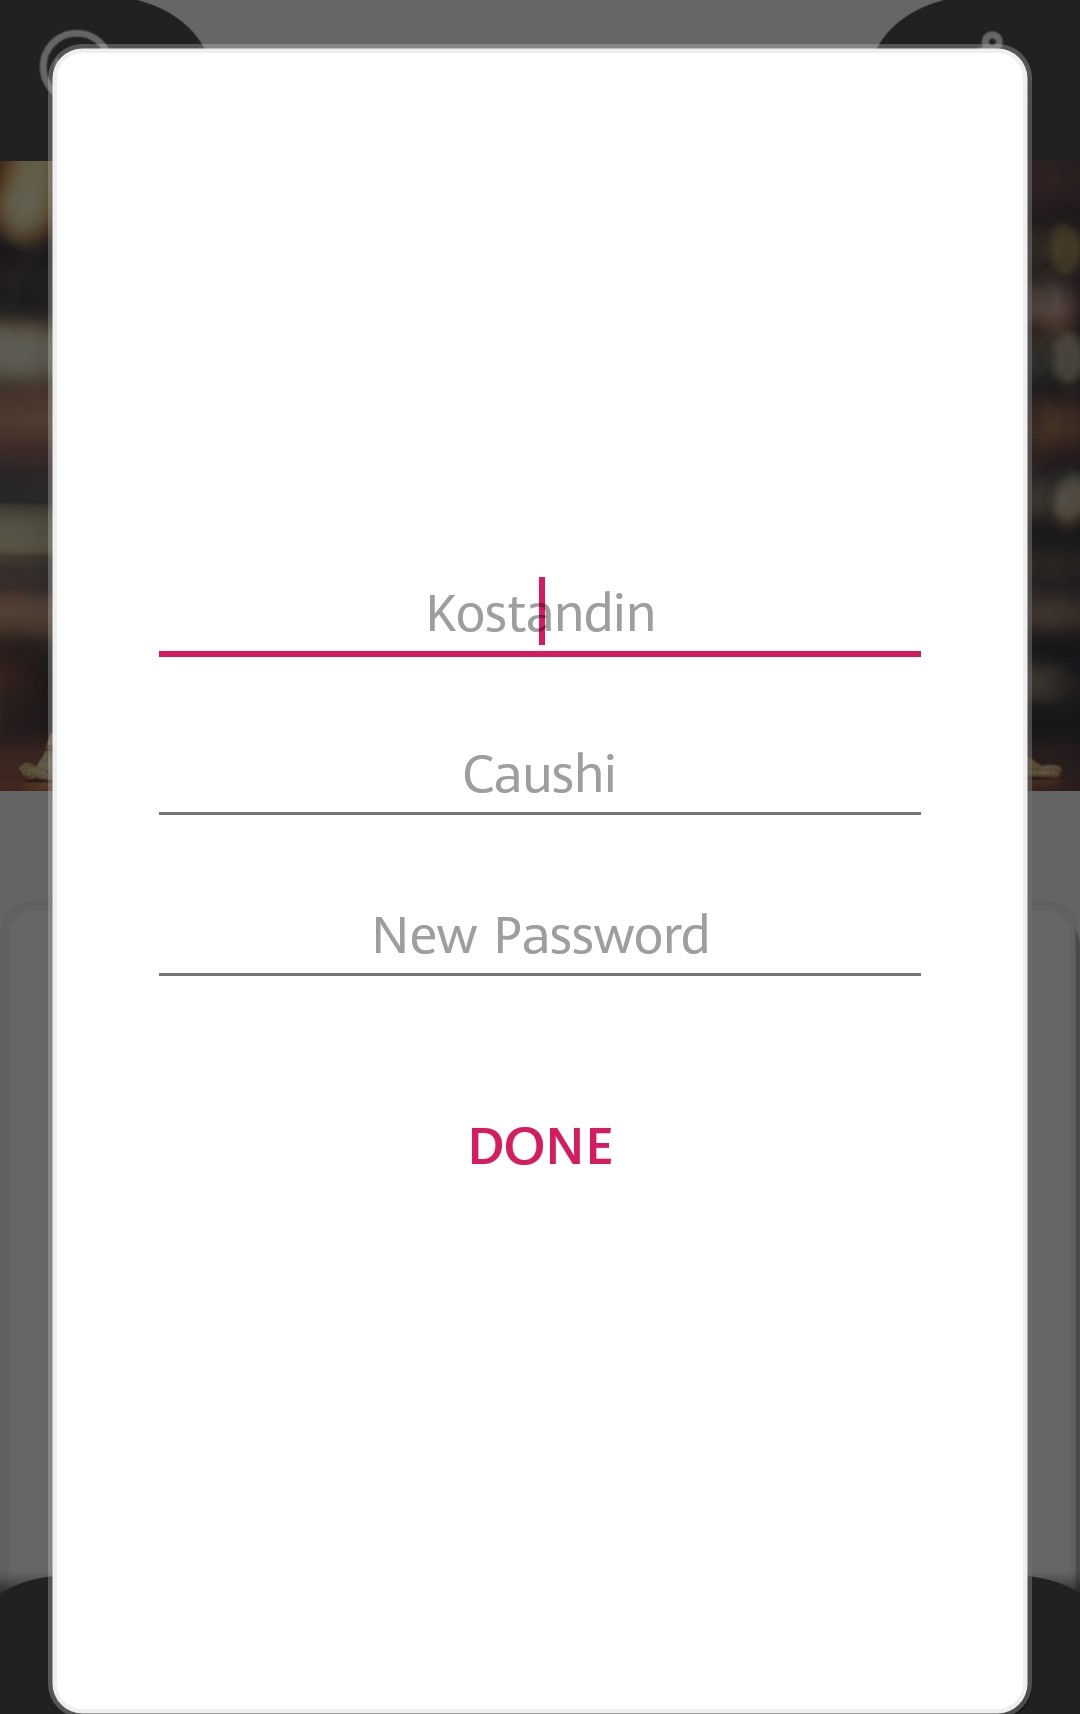
\includegraphics[scale=0.15]{Images/UI/Profile/3}
	\caption{Profile - UI}
\end{figure}

\newpage
\mysubsubsection{Confirm Reservation / Book Returned (EasyLib - Librarian)}
On the Librarian side, he can open the "Book Activity" scanning a qr-code and retrieving book all the book information and the list of all the Reservations for that one.\par
Based on the status of each reservation, different buttons are shown : if the book is already physically taken from the library than just the "Returned" button is shown; otherwise 2 buttons are shown "Reserve" that confirms the user reservations and sets the status to "Taken", or "Remove" that removes the reservation.\par
The images underneath shows the portrait and landscape orientation of this activity on tablet.
\vspace*{1cm}
\begin{figure}[H]
	\centering
	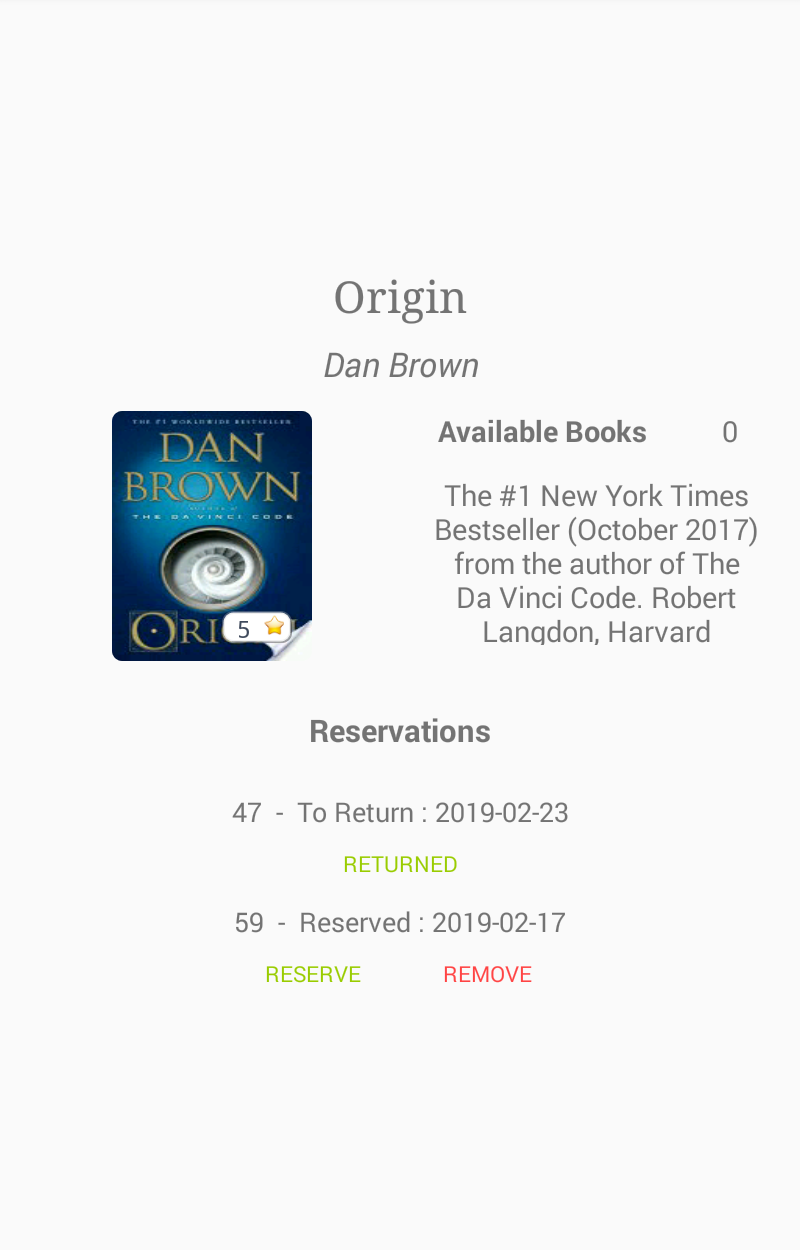
\includegraphics[scale=0.2]{Images/UI/Librarian/1}
	\hspace{0.5cm}
	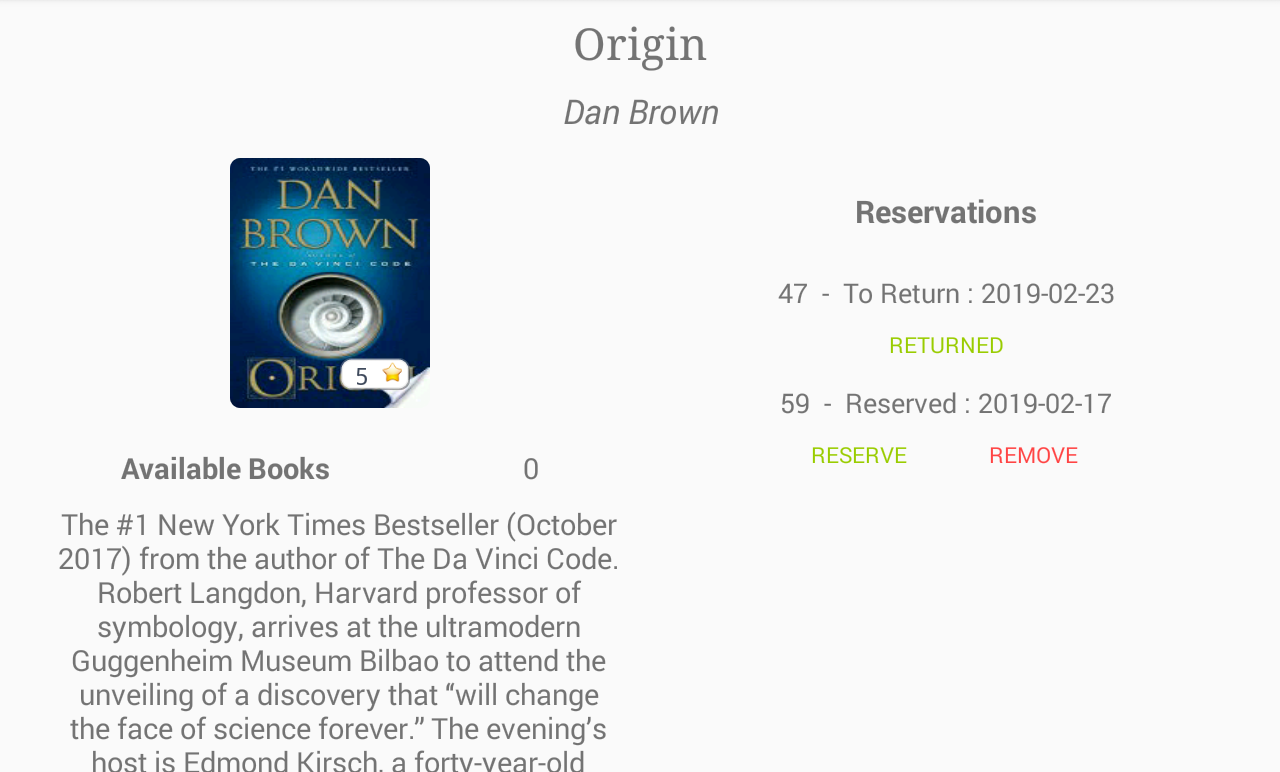
\includegraphics[scale=0.2]{Images/UI/Librarian/2}
	\caption{Confirm Reservation / Book Returned (EasyLib - Librarian) - UI}
\end{figure}